\chapter{输入模型：态制备与块编码}
\label{ch:lec06}

\begin{objectives}
\begin{itemize}[leftmargin=1.4em,nosep]
  \item 将态制备 (state preparation) 谕示 (oracle) 描述为\emph{向量}输入模型，并说明
        它在何时可以被高效实现。
  \item 将块编码 (block encoding) 定义为\emph{矩阵}输入模型，并读出其次归一化因子
        $\alpha$、辅助比特 (ancilla) 数目 $a$ 与误差 $\epsilon$。
  \item 将块编码作用于已制备的态上以执行\emph{矩阵--向量乘法}，并从 $\alpha$ 与输出范数
        读出其代价。
  \item 通过\emph{矩阵加法}、\emph{向量加法}与\emph{矩阵--矩阵乘法}组合输入模型，追踪
        $\alpha$ 与辅助比特数目如何复合。
  \item 从取值谕示与位置谕示构造 $1$-稀疏与 $s$-稀疏矩阵的块编码。
  \item 区分 Hermitian 块编码与一般块编码，并解释为什么这一区分对 qubitization 很重要。
  \item 认识一般投影子形式 $A=\alpha\,\Pi'\,U_A\,\Pi$ 中的块编码关系，它在计算基之外同样
        成立。
\end{itemize}
\end{objectives}

第~I~部分将量子态与酉线路视为基本对象。第~II~部分转向\emph{量子数值线性代数}：求解线性方程组、
作用矩阵函数、模拟动力学。每一个这样的任务都始于同一个问题——\emph{输入模型}：一个矩阵
$A\in\C^{N\times N}$（其中 $N=2^n$），它一般\emph{不是}酉的且可能是稠密的，如何进入一台量子
计算机，而后者唯一的原生操作却是酉的？本讲发展支撑整个 QNLA 工具箱的两种答案。第一种，
\emph{态制备谕示}，将一个经典向量加载到量子态的振幅中，是线性方程组右端项的输入模型。第二种，
\emph{块编码}，将 $A$（经重标度后）嵌入为一个更大的酉算符 $U_A$ 的左上角；它是矩阵本身的输入
模型，也是酉算符线性组合 (LCU, \cref{ch:lec07})、qubitization 与量子信号处理
(QSP, \cref{ch:lec08})、量子奇异值变换 (QSVT, \cref{ch:lec09}) 以及量子线性方程组求解器
(\cref{ch:lec10}) 所共同构建于其上的单一抽象。我们给出其定义，用\emph{次归一化因子} $\alpha$
量化其代价，并从一对谕示——一个给出取值、一个给出非零位置——显式构造稀疏矩阵的块编码。全文中，
$A$ 是一个 $n$ 比特矩阵，$\norm{A}$ 表示谱（算符）范数。

\section{态制备谕示}
\label{sec:lec06-1}

许多算法都相对于一个固定的输入向量而提出：线性方程组问题 $Ax=b$ 需要右端项 $b$；基态能量估计
(\cref{sec:lec05-1}) 需要一个初始猜测 $\ket{\phi}$；一个蒙特卡洛估计量被编码在一个已制备的振幅
中 (\cref{sec:lec05-2})。在每一种情形下，该向量都必须被加载到一个 $n$ 比特寄存器的振幅中。这就是
向量输入模型。

\begin{definition}[态制备谕示]
\label{def:lec06-sp}
设 $u\in\C^{N}$ 是一个非零向量，其归一化版本为
$\ket{u}=u/\norm{u}_2=\sum_{i=0}^{N-1}u_i\ket{i}/\norm{u}_2$。$u$ 的一个
\emph{态制备谕示}是一个 $n$ 比特酉算符 $O_u$，满足
\begin{equation}
  O_u\ket{0^n}=\ket{u}.
  \label{eq:lec06-sp}
\end{equation}
若 $O_u$ 可由一个规模为 $\poly(n)=\polylog(N)$ 的线路实现，则称该谕示是\emph{高效的}。
\end{definition}

归一化之后只有 $u$ 的方向得以保留；范数 $\norm{u}_2$ 是一个经典标量，必须单独追踪（例如，它会
作为线性方程组解的标度重新出现）。本质的微妙之处在于，\eqref{eq:lec06-sp} 很容易\emph{写出来}，
但并非总能廉价地\emph{实现}。

\begin{proposition}[精确振幅加载的代价]
\label{prop:lec06-sp}
对任意 $\ket{u}\in\C^{N}$，存在一个态制备酉算符 $O_u$ 满足 \eqref{eq:lec06-sp}，它使用
$\bigo(N)=\bigo(2^n)$ 个初等门且不需要辅助比特。一般而言，对最坏情形的 $\ket{u}$，这一代价不能
降到 $\Omega(2^n/n)$ 个门以下。
\end{proposition}

\begin{proof}[证明概要]
通过一系列受控单比特旋转来制备 $\ket{u}$，每个比特一个，这些旋转在已设定的比特的条件下逐步建立起
振幅。具体地，第一个比特被旋转，使其两个分支的概率匹配 $u$ 在第一比特为 $0$ 与为 $1$ 的那些态上的
总权重；在该比特的条件下，第二个比特被旋转以再次分割权重；如此继续。这棵树的第 $k$ 层需要
$2^{k-1}$ 个受控旋转（每个分支一个），因此总数为
$\sum_{k=1}^{n}2^{k-1}=2^{n}-1=\bigo(N)$ 个旋转，每个旋转的相位角与幅值角都从 $\abs{u_i}^2$ 与
$\arg u_i$ 的部分和中读出。至于下界，一般的 $\ket{u}$ 携带 $\Theta(2^n)$ 个独立实参数，而 $n$ 个
比特上由 $g$ 个两比特门构成的线路只有 $\bigo(g)$ 个连续参数；匹配参数个数迫使 $g=\Omega(2^n/n)$。
\end{proof}

\begin{figure}[ht]
\centering
\begin{tikzpicture}[every node/.style={font=\scriptsize},level distance=11mm,
  level 1/.style={sibling distance=34mm},level 2/.style={sibling distance=17mm},
  level 3/.style={sibling distance=8.5mm},
  rot/.style={circle,draw,fill=blue!8,inner sep=1.6pt}]
\node[rot]{}
  child{node[rot]{}
     child{node[rot]{} child{node{$u_0$}} child{node{$u_1$}}}
     child{node[rot]{} child{node{$u_2$}} child{node{$u_3$}}}
     edge from parent node[above left,inner sep=1pt]{$0$}}
  child{node[rot]{}
     child{node[rot]{} child{node{$u_4$}} child{node{$u_5$}}}
     child{node[rot]{} child{node{$u_6$}} child{node{$u_7$}}}
     edge from parent node[above right,inner sep=1pt]{$1$}};
\node[anchor=west,font=\scriptsize,gray] at (3.2,0){$1$ 个旋转};
\node[anchor=west,font=\scriptsize,gray] at (3.2,-1.1){$2$ 个旋转};
\node[anchor=west,font=\scriptsize,gray] at (3.2,-2.2){$4$ 个旋转};
\end{tikzpicture}
\caption{\cref{prop:lec06-sp} 的精确加载器作为一棵受控旋转的二叉树（$n=3$）。每个圆圈是一个单比特
$R_y$，它在上方比特的条件下把存留的概率质量在其 $0$-分支与 $1$-分支之间分配；第 $k$ 层携带
$2^{k-1}$ 个这样的旋转，共计 $2^n-1$ 个。$2^n$ 个叶子就是振幅 $u_i$。一般的 $\ket u$ 独立地固定全部
$2^n$ 个叶子，这正是为何没有线路能胜过 $\Omega(2^n/n)$ 个门。}
\label{fig:lec06-sptree}
\end{figure}

\cref{prop:lec06-sp} 的信息是，\emph{任意}振幅加载是指数级昂贵的，并且就其本身而言会摧毁任何量子
加速的希望。只有对\emph{结构化}向量，高效态制备才是可能的。

\begin{example}[态制备何时高效]
\label{exa:lec06-spgood}
有四大类结构允许 $\polylog(N)$ 规模的制备。
\begin{itemize}[leftmargin=1.4em,nosep]
  \item \emph{乘积（无纠缠）态。}若 $\ket{u}=\bigotimes_{k=1}^{n}
        \ket{v_k}$，其中每个 $\ket{v_k}$ 是单个比特，则 $O_u=\bigotimes_k
        R_k$ 是 $n$ 个单比特旋转。均匀叠加
        $\Hgate^{\otimes n}\ket{0^n}$ 是 $\ket{v_k}=\ket{+}$ 的特殊情形。
  \item \emph{可高效积分的分布。}若 $\abs{u_i}^2=p(i)$，其中 $p$ 是一个累积分布可经典计算的
        概率密度，则 Grover--Rudolph 程序用 $\bigo(n)$ 个受控旋转加载 $\ket{u}$，每个旋转角由 $p$
        在一个二进分子区间上的积分设定。
  \item \emph{稀疏向量。}若 $u$ 只有 $d=\poly(n)$ 个非零元，其指标与取值已知，则 $\ket{u}$ 可用
        $\bigo(dn)$ 个门制备，办法是一次加载一个振幅，共 $d$ 个。
  \item \emph{矩阵乘积态。}若 $\ket{u}$ 是一个键维数 (bond dimension) 为 $\chi$ 的矩阵乘积态
        （一个 $\mathrm{MPS}$，即一维张量网络），则它可由 $n$ 个顺序酉算符\emph{精确}地制备，每个
        作用于 $\lceil\log_2\chi\rceil+1$ 个比特——总共 $\bigo(n\,\poly(\chi))$ 个门。上面的乘积态
        条目是 $\chi=1$ 的特殊情形。键维数有界的态是第~IV~部分 (\cref{ch:lec15}) 的主题；其高维类比
        (PEPS) 一般\emph{不}可高效制备。
\end{itemize}
当没有这样的结构可用时，人们可以退而求助于量子随机存取存储器 (QRAM)，它以 $\bigo(N)$ 硬件为代价，
在 $\bigo(n)$ \emph{深度}内提供 $O_u$；QRAM 是否是一种现实的资源仍是一个悬而未决的争论。
\end{example}

我们把这四类分别落实为具体例子，并给出其制备线路。

\begin{example}[乘积态]
\label{exa:lec06-prod}
取三量子比特乘积态
$\ket{u}=\ket+\otimes\ket0\otimes\bigl(\cos\tfrac\pi8\ket0+\sin\tfrac\pi8\ket1\bigr)$。
由于它可因式分解，$O_u=\Hgate\otimes\id\otimes R_y(\tfrac\pi4)$ 就是每条线上一个
单量子比特门（中间那个比特上没有门）——没有两量子比特门，因而没有纠缠。
\begin{center}
\begin{quantikz}
  \lstick{$\ket0$} & \gate{\Hgate}        & \qw \\
  \lstick{$\ket0$} & \qw                  & \qw \\
  \lstick{$\ket0$} & \gate{R_y(\pi/4)}    & \qw
\end{quantikz}
\end{center}
乘积态的 $n$ 个振幅只携带 $n$ 个独立角度，故 $n$ 个旋转即足够；均匀叠加
$\Hgate^{\otimes n}\ket{0^n}$ 就是其中每个门都是 Hadamard 的情形。
\end{example}

\begin{remark}[Grover--Rudolph 程序]
\label{rem:lec06-gr}
第二类是加载概率分布的主力，因此值得详细说明。假设目标具有实非负振幅
$\ket{u}=\sum_{i}\sqrt{p(i)}\,\ket{i}$，它是 $[0,1)$ 上密度 $p$ 到 $2^{n}$ 个二进分格子的离散化
（指标 $i$ 是二进制小数 $0.i_1i_2\cdots i_n$）。Grover--Rudolph 逐比特地构建 $\ket{u}$，在下降过程中
分割概率质量。一旦前 $k$ 个比特被固定，它们就命名一个宽度为 $2^{-k}$ 的二进分区间 $I$；作用于第
$k{+}1$ 个比特的旋转是
\[
  R_y(\theta_I)\ket0=\cos\tfrac{\theta_I}{2}\ket0+\sin\tfrac{\theta_I}{2}\ket1,
  \qquad
  \cos^{2}\tfrac{\theta_I}{2}=\frac{\int_{I_{\mathrm{left}}}p}{\int_{I}p},
\]
于是两个分支恰好继承 $I$ 左半与右半的质量（\cref{fig:lec06-gr}）。在所有 $n$ 层上叠套展开，
$\ket i$ 上的平方振幅等于格子质量 $\int_{\text{cell }i}p\approx p(i)$，正如所要求的。
\begin{figure}[ht]
\centering
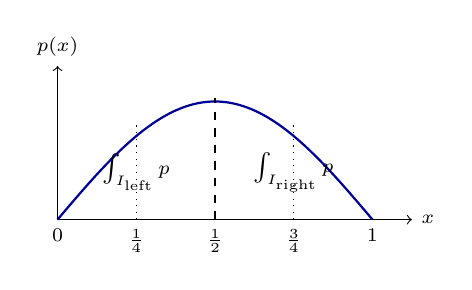
\begin{tikzpicture}[scale=1]
  \draw[->](0,0)--(4.5,0) node[right,font=\scriptsize]{$x$};
  \draw[->](0,0)--(0,1.95) node[above,font=\scriptsize]{$p(x)$};
  \draw[thick,blue!60!black,domain=0:1,smooth,variable=\x,samples=50]
       plot ({4*\x},{1.5*sin(180*\x)});
  \draw[dashed](2,0)--(2,1.55);
  \draw[dotted](1,0)--(1,1.25);  \draw[dotted](3,0)--(3,1.25);
  \foreach \px/\lab in {0/$0$,1/$\frac14$,2/$\frac12$,3/$\frac34$,4/$1$}
     \node[font=\scriptsize,below] at (\px,0){\lab};
  \node[font=\scriptsize] at (1,0.6){$\int_{I_{\mathrm{left}}}p$};
  \node[font=\scriptsize] at (3,0.6){$\int_{I_{\mathrm{right}}}p$};
\end{tikzpicture}
\caption{Grover--Rudolph 以二进分二分法分割质量。第一个比特的第一层旋转取
$\cos^2(\theta/2)=\int_{I_{\mathrm{left}}}p\big/\int_{[0,1)}p$（虚线分隔在 $\tfrac12$ 处）；随后每个
比特二分存留的区间（点线分隔在 $\tfrac14,\tfrac34$ 处），故第 $k$ 层携带 $2^{k-1}$ 个条件旋转。}
\label{fig:lec06-gr}
\end{figure}

关键在于\emph{为什么这只花 $\bigo(n)$ 个旋转}。在第 $k$ 层为 $2^{k-1}$ 个区间各硬编码一个单独的角度
会花掉 $\sum_{k=1}^{n}2^{k-1}=\bigo(2^{n})$——并不比一般的 \cref{prop:lec06-sp} 更好。增益完全
依赖于积分 $\int_{I}p$ 是\emph{经典可高效计算}这一假设：人们不去枚举区间，而是把已设定的比特
$i_1\cdots i_k$ 保存在一个寄存器中，由它们\emph{相干地}计算角度 $\theta$（在一个辅助比特上用 $p$ 的
累积分布做算术），作用一个由该寄存器所持角度决定的旋转，然后反计算。每一层都是一个这样的
$\poly(n)$ 门块，而共有 $n$ 层。一个告诫 (Herbert, 2021)：若积分只能由蒙特卡洛\emph{估计}而不能以
封闭形式求值，则采样代价可能抵消所加载态本应带来的那一份加速——因此该方法只对真正可积的密度
（对数凹、高斯及类似者）才有收益。
\end{remark}

\begin{example}[高效可积：四点上的 Grover--Rudolph]
\label{exa:lec06-grex}
在 $n=2$ 个量子比特上加载 $p=(3,1,1,3)/8$，即
$\ket{u}=\tfrac1{\sqrt8}\bigl(\sqrt3\,\ket{00}+\ket{01}+\ket{10}+\sqrt3\,\ket{11}\bigr)$。
以 $q_1$ 为最高有效位，两个半区 $\{00,01\}$ 与 $\{10,11\}$ 各携带相等的质量
$\tfrac12$，故第一层的角度满足 $\cos^2(\theta_1/2)=\tfrac12$，即对 $q_1$ 施加
$R_y(\pi/2)=\Hgate$。在 $q_1$ 的条件下，第二层的角度再把每一半区细分：
$q_1{=}0$ 给出 $\cos^2(\theta/2)=p_{00}/(p_{00}{+}p_{01})=\tfrac34$，故为 $R_y(\pi/3)$；
$q_1{=}1$ 给出 $p_{10}/(p_{10}{+}p_{11})=\tfrac14$，故为 $R_y(2\pi/3)$。于是第二层是一个
\emph{一致受控}（uniformly controlled）旋转——$q_1$ 的每个取值对应一个角度：
\begin{center}
\begin{quantikz}
  \lstick{$q_1:\ket0$} & \gate{\Hgate} & \octrl{1}          & \ctrl{1}            & \qw \\
  \lstick{$q_2:\ket0$} & \qw           & \gate{R_y(\pi/3)}  & \gate{R_y(2\pi/3)}  & \qw
\end{quantikz}
\end{center}
$\ket{00}$ 上的振幅为 $\cos\tfrac\pi4\cos\tfrac\pi6
=\tfrac1{\sqrt2}\cdot\tfrac{\sqrt3}2=\sqrt3/\sqrt8=\sqrt{p_{00}}$，正如所应。对于光滑的
密度，每一层的角度是在辅助比特上由 $\int_I p$ \emph{计算}得到、而非硬编码的，这正是
\cref{rem:lec06-gr} 的内容。
\end{example}

\begin{example}[稀疏向量]
\label{exa:lec06-sparsevec}
三量子比特态 $\ket{u}=\tfrac1{\sqrt2}(\ket{000}+\ket{101})$ 只有 $d=2$ 个非零振幅。
两个字上的相等权重由一个 Hadamard 和一个 $\CNOT$ 产生：对 $q_0$ 施加 $\Hgate$ 得到
$\tfrac1{\sqrt2}(\ket{000}+\ket{100})$，再用 $\CNOT_{q_0\to q_2}$ 翻转 $\ket{1\cdots}$
分支的最后一位，得到 $\ket{101}$。
\begin{center}
\begin{quantikz}
  \lstick{$q_0:\ket0$} & \gate{\Hgate} & \ctrl{2} & \qw \\
  \lstick{$q_1:\ket0$} & \qw           & \qw      & \qw \\
  \lstick{$q_2:\ket0$} & \qw           & \targ{}  & \qw
\end{quantikz}
\end{center}
一般而言，$d$-稀疏向量逐个振幅地加载：用 $\bigo(n)$ 个门寻址 $d$ 个位置中的每一个并
设定其大小与相位，共计 $\bigo(dn)$ 个门。
\end{example}

\begin{example}[矩阵乘积态：GHZ]
\label{exa:lec06-mps}
GHZ 态 $\ket{u}=\tfrac1{\sqrt2}(\ket{000}+\ket{111})$ 是最简单的非平凡矩阵乘积态，键维数
$\chi=2$。它的顺序式 MPS 制备就是教科书上的线路——对第一个量子比特施加 Hadamard，再接
一条沿寄存器传递键指标的 $\CNOT$ 链：
\begin{center}
\begin{quantikz}
  \lstick{$q_0:\ket0$} & \gate{\Hgate} & \ctrl{1} & \qw      & \qw \\
  \lstick{$q_1:\ket0$} & \qw           & \targ{}  & \ctrl{1} & \qw \\
  \lstick{$q_2:\ket0$} & \qw           & \qw      & \targ{}  & \qw
\end{quantikz}
\end{center}
每个门作用在 $\lceil\log_2\chi\rceil+1=2$ 个量子比特上，共有 $n-1$ 个，与
$\bigo(n\,\poly(\chi))$ 的计数相符；对更大的 $\chi$，这些 $\CNOT$ 换成 \cref{ch:lec15}
中的键酉算符。
\end{example}

\begin{remark}[一般 $n$ 的键维数：GHZ（$\chi=2$）与 Dicke（$\chi=3$）]
\label{rem:lec06-mpschi}
这两族都可推广到任意数目的量子比特，键指标恰好携带左块跨过某一割缝时必须传给右块的
那部分信息。

\emph{键维数 $2$（GHZ）。} $n$ 量子比特 GHZ 态
$\tfrac1{\sqrt2}(\ket0^{\otimes n}+\ket1^{\otimes n})$ 是具有对角 $2\times2$ 张量
$A^0=\proj0$、$A^1=\proj1$，以及边界余向量 $\bra{L}=\bra0+\bra1$、
$\ket{R}=\ket0+\ket1$ 的 MPS：乘积 $A^{x_1}\cdots A^{x_n}$ 仅当所有比特一致时才不为零
（任何混合串都含有一个因子 $\proj0\proj1=0$），只剩下两个均匀项。键只传递一个比特
——属于哪一支——故 $\chi=2$。顺序式线路为一个 $\Hgate$ 加上一条由 $n-1$ 个最近邻
$\CNOT$ 构成的链（此处以 $n=4$ 为例；那个被``携带''的单一量子比特\emph{就是}键）：
\begin{center}
\begin{quantikz}
  \lstick{$q_1:\ket0$} & \gate{\Hgate} & \ctrl{1} & \qw      & \qw      & \qw \\
  \lstick{$q_2:\ket0$} & \qw           & \targ{}  & \ctrl{1} & \qw      & \qw \\
  \lstick{$q_3:\ket0$} & \qw           & \qw      & \targ{}  & \ctrl{1} & \qw \\
  \lstick{$q_4:\ket0$} & \qw           & \qw      & \qw      & \targ{}  & \qw
\end{quantikz}
\end{center}

\emph{键维数 $3$（Dicke）。} 权重为 $2$ 的 Dicke 态
$\ket{D^n_2}=\binom n2^{-1/2}\sum_{\abs x=2}\ket x$ 是这样一个 MPS：其键指标
$m\in\{0,1,2\}$ 记录迄今已放置的 $1$ 的个数，张量为 $3\times3$ 的
\[
  A^0=\id_3,\qquad
  A^1=\begin{pmatrix}0&0&0\\ 1&0&0\\ 0&1&0\end{pmatrix},
\]
从起始键 $m=0$ 读到终止键 $m=2$。由于 $A^0$ 因子都是单位阵，乘积约化为
$(A^1)^{\abs x}$，而 $\bra{2}(A^1)^{\abs x}\ket0=\delta_{\abs x,2}$ 恰好挑出权重为 $2$ 的
串。跨过任一割缝，左块都必须宣告它已用掉多少个 $1$——$0$、$1$ 或 $2$，三条可区分的
消息——故施密特秩、也即键维数，为 $3$。（更一般地，$\ket{D^n_k}$ 有 $\chi=k+1$：键
一直计数到 $k$。）

\emph{代价。} 一个 $\chi$-MPS 由 $n$ 个顺序酉算符制备，每个作用在
$\lceil\log_2\chi\rceil+1$ 个量子比特上：GHZ（$\chi=2$，即上面的 $\Hgate$ 加 $\CNOT$
链）用两量子比特门，$\ket{D^n_2}$（$\chi=3$，一个 $\lceil\log_2 3\rceil=2$ 比特的键
寄存器依次与每个发射出的量子比特耦合）用三量子比特门——两种情形都是 $\bigo(n)$ 个门。
通用的单步复用键寄存器并发射一个物理量子比特：
\begin{center}
\begin{quantikz}
  \lstick{键 $\ket0$}   & \gate[3]{V_k} & \qw \\
  \lstick{键 $\ket0$}   &               & \qw \\
  \lstick{新鲜 $\ket0$} &               & \rstick{$q_k$}\qw
\end{quantikz}
\end{center}
依次施加 $V_1,\dots,V_n$ 并最终把键寄存器复位到 $\ket{00}$，便得到 $\ket{D^n_2}$；当
$\chi=2$ 时键是单个量子比特，每个 $V_k$ 即上面链中的那个两量子比特门。
\end{remark}

\begin{example}[显式的 Dicke 态 $\ket{D^3_2}$ 与 $\ket{D^4_2}$]
\label{exa:lec06-dicke34}
顺序式（MPS）制备背后的递推把第一个比特剥离出来：
\[
  \ket{D^n_k}=\sqrt{\tfrac{n-k}{n}}\,\ket0\otimes\ket{D^{n-1}_k}
             +\sqrt{\tfrac{k}{n}}\,\ket1\otimes\ket{D^{n-1}_{k-1}},
\]
因为在 $\binom nk$ 个权重为 $k$ 的串中，有 $(n-k)/n$ 的比例以 $0$ 开头、$k/n$ 的比例以 $1$ 开头。
将它展开即得显式的小线路。

\emph{$n=3$。} 以 $\ket{D^2_2}=\ket{11}$、$\ket{D^2_1}=\tfrac1{\sqrt2}(\ket{01}+\ket{10})$，
\[
  \ket{D^3_2}=\sqrt{\tfrac13}\,\ket0\ket{11}+\sqrt{\tfrac23}\,\ket1\ket{D^2_1}
             =\tfrac1{\sqrt3}\bigl(\ket{011}+\ket{101}+\ket{110}\bigr).
\]
分三步制备：对 $q_1$ 作 $R_y(\theta_1)$，$\theta_1=2\arccos\sqrt{\tfrac13}$（使
$q_1\mapsto\sqrt{\tfrac13}\ket0+\sqrt{\tfrac23}\ket1$）；在 $q_1{=}0$ 的条件下把 $q_2q_3$ 置为
$\ket{11}$；在 $q_1{=}1$ 的条件下在 $q_2q_3$ 上制备 $\ket{D^2_1}$（一个 $\Hgate$ 和一个 $\CNOT$，至多
差一次比特翻转）。由于对 $n=3$ 权重二是权重一的\emph{补}，等价地
$\ket{D^3_2}=X^{\otimes3}\ket{W_3}$，其中 $\ket{W_3}=\tfrac1{\sqrt3}(\ket{100}+\ket{010}+\ket{001})$。

\emph{$n=4$。} 此时 $\tfrac{n-k}{n}=\tfrac{k}{n}=\tfrac12$，故第一个旋转是 Hadamard：
\[
  \ket{D^4_2}=\tfrac1{\sqrt2}\,\ket0\ket{D^3_2}+\tfrac1{\sqrt2}\,\ket1\ket{W_3}
  =\tfrac1{\sqrt6}\bigl(\ket{0011}+\ket{0101}+\ket{0110}+\ket{1001}+\ket{1010}+\ket{1100}\bigr),
\]
这里用到 $\ket{D^3_1}=\ket{W_3}$。线路是：对 $q_1$ 作 $\Hgate$，再在 $q_1$ 控制下于 $q_2q_3q_4$ 上制备
——$q_1{=}0$ 时制备 $\ket{D^3_2}$，$q_1{=}1$ 时制备 $\ket{W_3}$——每个都是 $n=3$ 情形的三比特块。这就是
Bärtschi--Eidenbenz 递推；其扁平（非递归）版本复用单个``运行权重''辅助比特，达到
\cref{rem:lec06-mpschi} 所述的 $\bigo(kn)$ 门、$\bigo(n)$ 深度的线路。
\end{example}

\begin{example}[用相位梯度编码 $\sin(x_1+\cdots+x_d)$]
\label{exa:lec06-sinvec}
一个\emph{并非}各寄存器函数之乘积的函数，只要它的\emph{相位}是可乘的，仍可廉价地加载。
考虑 $d$ 个 $m$ 比特寄存器（每轴 $N=2^m$）上的实向量
$\ket\psi\propto\sum_{\mathbf x}\sin(x_1+\cdots+x_d)\,\ket{x_1}\cdots\ket{x_d}$。尽管
$\sin(\sum_k x_k)$ 不可因式分解，其相位却可以：
$\ee^{\ii\sum_k x_k}=\prod_{k}\prod_{b=0}^{m-1}\ee^{\ii 2^b(x_k)_b}$，于是\emph{相位梯度态}
\[
  \ket g=\sum_{\mathbf x}\ee^{\ii\sum_k x_k}\ket{\mathbf x}
   =\bigotimes_{k=1}^{d}\bigotimes_{b=0}^{m-1}\bigl(\ket0+\ee^{\ii 2^b}\ket1\bigr)
\]
是一个\emph{乘积}态——在 $dm$ 个量子比特的每一个上施加一个单比特相位
$P(2^b)=\diag(1,\ee^{\ii2^b})$（在一层 Hadamard 之后），没有任何纠缠门。\emph{相位梯度}
这一名称指的是相位在基上的分布方式：$\ket{\mathbf x}$ 的振幅携带相位 $\sum_k x_k$，它关于每个整数
坐标\emph{线性}增长——一个恒定的斜坡、即梯度——而比特 $b$ 贡献二进制加权的步长 $2^b$，这正是 QFT 与
Draper 加法器（\cref{sec:lec04-qftadder}）所用的那道相位阶梯。利用
$\sin\theta=(\ee^{\ii\theta}-\ee^{-\ii\theta})/2\ii$，
\[
  \ket\psi=\frac{1}{2\ii}\bigl(\ket g-\ket{g^{*}}\bigr),\qquad
  \ket{g^{*}}=\bigotimes_{k,b}\bigl(\ket0+\ee^{-\ii2^b}\ket1\bigr),
\]
这是一个两项组合，可用一个标志比特像 Hadamard 检验（\cref{sec:lec04-1}）那样提取：在数据上
制备均匀叠加、在标志上制备 $\ket+$，施加\emph{受标志控制}的相位梯度 $\Phi^{\pm}$（标志为
$\ket0$ 时相位取 $+2^b$，为 $\ket1$ 时取 $-2^b$），再对标志作 $\Hgate$ 并测量。
\begin{center}
\begin{quantikz}
  \lstick{$\ket0$ \,\scriptsize(标志)}  & \gate{\Hgate}              & \gate[2]{\Phi^{\pm}} & \gate{\Hgate} & \meter{} \\
  \lstick{$\ket{0^{dm}}$ \,\scriptsize(数据)} & \gate{\Hgate^{\otimes dm}} &                      & \qw           & \qw
\end{quantikz}
\end{center}
测得 $1$ 使数据处于归一化的正弦态
$\propto\sum_{\mathbf x}\sin(\sum_k x_k)\ket{\mathbf x}$；测得 $0$ 则给出\emph{余弦}态
$\propto\sum_{\mathbf x}\cos(\sum_k x_k)\ket{\mathbf x}$，即错误的向量——只需丢弃它并重跑这个（廉价的）
线路。标志读到 $1$ 的概率为 $N^{-d}\sum_{\mathbf x}\sin^2(\sum_k x_k)\approx\tfrac12$，故期望的尝试次数
为 $\bigo(1)$（约两次）；等价地，对标志作一轮振幅放大（\cref{ch:lec03}）即可使该制备\emph{确定化}、
无需重复。总代价是 $\bigo(dm)$ 个单比特与受控相位门——无需振幅加载、无需算术。同样的手法可编码任何线性型
$\sum_k a_k x_k$ 的 $\sin$ 或 $\cos$（相位取 $\ee^{\pm\ii a_k2^b}$）；只有取虚部这一步需要标志，
因为乘积 $\prod_k f_k(x_k)$ 本就可分解为单寄存器的制备。
\end{example}

\begin{remark}[可分离与相位多项式的变体]
\label{rem:lec06-phasepoly}
同样的想法按指数如何嵌入量子比特对相关编码作出分类。
\begin{itemize}[leftmargin=1.4em,nosep]
  \item \emph{可分离（最易）：$\ee^{\sum_k a_k x_k}$。}线性型的实指数\emph{可因式分解}，
        $\ee^{\sum_k a_k x_k}=\prod_{k,b}\ee^{a_k 2^b (x_k)_b}$，于是
        $\sum_{\mathbf x}\ee^{\sum_k a_k x_k}\ket{\mathbf x}
        =\bigotimes_{k,b}\bigl(\ket0+\ee^{a_k 2^b}\ket1\bigr)$ 是一个\emph{乘积}态——每个
        量子比特上一个单比特旋转 $R_y(\theta_{k,b})$，其中 $\theta_{k,b}$ 使寄存器 $k$ 的第 $b$ 个
        比特倾斜为 $R_y(\theta_{k,b})\ket0\propto\ket0+\ee^{a_k 2^b}\ket1$，即
        $\tan(\theta_{k,b}/2)=\ee^{a_k 2^b}$，等价地 $\theta_{k,b}=2\arctan(\ee^{a_k 2^b})$；
        既无辅助比特也无纠缠门。（各振幅跨越双指数的量级，故通常对自变量重标度，如 $\ee^{-a_k x_k}$，以免
        态坍缩到单一角点。）
  \item \emph{相位多项式：$\sin(x_1x_2\cdots x_d)$。}此时指数是一个\emph{乘积}。按比特展开，
        $x_1\cdots x_d=\sum_{b_1,\dots,b_d}2^{b_1+\cdots+b_d}(x_1)_{b_1}\cdots(x_d)_{b_d}$，
        故 $\ee^{\ii x_1\cdots x_d}$ 是 $m^d$ 个多重受控相位
        $C^{d-1}P\bigl(2^{\sum_k b_k}\bigr)$ 之积（仅当 $d$ 个被选比特全为 $1$ 时才施加相位）。
        于是 $\ket g=\sum_{\mathbf x}\ee^{\ii x_1\cdots x_d}\ket{\mathbf x}$ 是
        $\Hgate^{\otimes dm}$ 后接那 $m^d$ 个受控相位——有纠缠，但对固定 $d$ 为 $\poly(m)$——而
        $\sin(x_1\cdots x_d)$ 是其虚部，用 \cref{exa:lec06-sinvec} 的单标志步骤读出。代价关于
        $d$ 是指数的（$d$ 次单项式的个数），这是真正多线性指数的代价。
\end{itemize}
一般地，若 $f(\mathbf x)=\ee^{\ii\varphi(\mathbf x)}$ 的实部或虚部、而 $\varphi$ 是一个多线性
相位多项式，则相位态是一层（多重）受控相位——每个单项式一个——而单个标志比特把复相位态
转为实的 $\sin/\cos$ 振幅向量。
\end{remark}

\begin{example}[径向振幅 $1/\lvert\mathbf x\rvert$ 作为高斯之和]
\label{exa:lec06-coulomb}
库仑型向量 $1/\lvert\mathbf x\rvert$（$\lvert\mathbf x\rvert=\sqrt{x_1^2+\cdots+x_d^2}$）
既不可分离、也非相位多项式——和的平方根同时挫败了这两种技巧。标准手段是一个恢复可分离性的
\emph{积分表示}：
\[
  \frac{1}{\lvert\mathbf x\rvert}
  =\frac{2}{\sqrt\pi}\int_0^\infty \ee^{-\lvert\mathbf x\rvert^2 t^2}\,dt
  =\frac{2}{\sqrt\pi}\int_0^\infty \prod_{k=1}^d \ee^{-x_k^2 t^2}\,dt
  \qquad(\mathbf x\neq0),
\]
其被积函数是一个\emph{可分离}的高斯函数。把 $t$ 离散化到几何网格 $\{t_q\}$ 并配以权重
$\{w_q\}$（高斯型求积，$Q=\bigo\bigl(\log\tfrac1\epsilon\,\log\tfrac{r_{\max}}{r_{\min}}\bigr)$
个节点即足够，Beylkin--Monzón），便化为乘积态的有限线性组合，
\[
  \sum_{\mathbf x}\frac{1}{\lvert\mathbf x\rvert}\ket{\mathbf x}
  \ \approx\ \sum_{q} w_q\,\bigotimes_{k=1}^{d}
     \Bigl(\sum_{x_k}\ee^{-x_k^2 t_q^2}\ket{x_k}\Bigr).
\]
这里 $\mathbf x=(x_1,\dots,x_d)$ 是一个格点的 $d$ 个空间\emph{坐标}——$d$ 个数据寄存器的内容，即我们
所叠加的变量——而 $t_q$ 是\emph{求积节点}（高斯的宽度），一张预先固定的、含 $Q$ 个数的经典列表；二者
不应混淆。每个一维高斯寄存器 $\sum_{x_k}\ee^{-x_k^2 t_q^2}\ket{x_k}$ 是一个\emph{高效可积}分布，由
Grover--Rudolph（\cref{exa:lec06-grex}）用 $\bigo(m)$ 个受控旋转制备；这 $Q$ 项则由
\cref{ch:lec07} 的向量加法（LCU）基本操作组合起来——一个 $\lceil\log_2 Q\rceil$ 比特的索引
寄存器由 $\mathrm{PREP}$ 加载 $\sqrt{w_q}$，一个 $\mathrm{SEL}$ 受索引控制地制备宽度为 $t_q$
的高斯乘积，最后对索引标志作后选择：
\begin{center}
\begin{quantikz}
  \lstick{$\ket{0^{\lceil\log Q\rceil}}$ \,\scriptsize(索引)} & \gate{\mathrm{PREP}} & \ctrl{1} & \gate{\mathrm{PREP}^{\dagger}} & \meter{} \\
  \lstick{$\ket{0^{dm}}$ \,\scriptsize(数据 $x_1,\dots,x_d$)}  & \qwbundle{dm}        & \gate{\mathrm{SEL}} & \qw                    & \qw
\end{quantikz}
\end{center}
其中 $\mathrm{SEL}=\sum_q\proj{q}\otimes O_q$，而 $O_q$ 制备
$\bigotimes_k(\sum_{x_k}\ee^{-x_k^2 t_q^2}\ket{x_k})$。总代价为 $\bigo(Qdm)$ 个门，索引标志被
测得的概率为
$\lVert\sum_{\mathbf x}\lvert\mathbf x\rvert^{-1}\ket{\mathbf x}\rVert^2/\lVert w\rVert_1^2$。
同样的高斯求和配方可编码任何具有已知一维变换的径向函数——$\lvert\mathbf x\rvert^{-s}$、
$\ee^{-\mu\lvert\mathbf x\rvert}$、汤川核 $\ee^{-\mu\lvert\mathbf x\rvert}/\lvert\mathbf x\rvert$——
并支撑着库仑相互作用的量子处理。
\end{example}

\begin{remark}[用算术加载实多项式振幅：$\sum_{i\neq j}x_ix_j$]
\label{rem:lec06-polyamp}
当目标振幅是一个\emph{实多项式}、而非某个相位的实部或虚部时，相位梯度技巧不再直接适用；
通用工具是\emph{计算–旋转–反计算}。取 $f(\mathbf x)=\sum_{i\neq j}x_ix_j$。先作代数化简，
\[
  \sum_{i\neq j}x_ix_j=\Bigl(\sum_i x_i\Bigr)^{\!2}-\sum_i x_i^{2}=S^2-Q,
\]
于是 $f$ 只需线性型 $S=\sum_i x_i$（一棵 $\bigo(\log d)$ 深的模加法器之树，
\cref{sec:lec04-qftadder}）以及可分离的平方和 $Q=\sum_i x_i^2$（对每个寄存器平方后相加）。
用可逆算术把 $f(\mathbf x)=S^2-Q$ 算入一个工作寄存器，再按寄存器所存之值施加旋转
$R_y\!\bigl(2\arcsin(f(\mathbf x)/F)\bigr)$（$F=\max_{\mathbf x}\abs{f(\mathbf x)}$）到一个
信号比特上，最后反计算工作寄存器：
\begin{center}
\begin{quantikz}
  \lstick{$\ket{\mathbf x}$ \,\scriptsize(数据)}   & \gate[2]{\textsc{arith}} & \qw          & \gate[2]{\textsc{arith}^{\dagger}} & \qw \\
  \lstick{$\ket{0}$ \,\scriptsize(工作)}           &                          & \gate[2]{R_y} &                                   & \qw \\
  \lstick{$\ket{0}$ \,\scriptsize(信号)}           & \qw                      &               & \qw                               & \qw
\end{quantikz}
\end{center}
这正是用可逆数据通路实现的 \eqref{eq:lec06-OA} 之条目谕示 $O_A$。方框 $\textsc{arith}$ 就是这条数据
通路：它读入数据寄存器 $\ket{\mathbf x}$，用普通的可逆整数算术把 $f(\mathbf x)$ 写入一个新鲜的工作
寄存器——一棵计算 $S=\sum_i x_i$ 的加法器树、对每个 $x_i^2$（以及 $S^2$）的平方电路、以及形成 $S^2-Q$
的减法器——使得 $\textsc{arith}\,\ket{\mathbf x}\ket0=\ket{\mathbf x}\ket{f(\mathbf x)}$。旋转 $R_y$
\emph{受工作寄存器所存之值控制}（一个按寄存器编码之角度的旋转，如 \cref{rem:lec06-gr}），而
$\textsc{arith}^{\dagger}$ 把同一数据通路反向运行，把工作寄存器清回 $\ket0$，不留下与数据纠缠的垃圾。
净效果使信号携带振幅 $f(\mathbf x)/F$，故在均匀数据态上对信号作后选择即得
$\propto\sum_{\mathbf x}f(\mathbf x)\ket{\mathbf x}$，用 $\poly(d,m)$ 个门。同一配方可加载任何高效可
计算的实振幅（唯一改变的是 $\textsc{arith}$）。

还有一种避开算术但为近似的相位态方案：由于每个 $x_ix_j$ 是双线性的，
$\ee^{\ii\theta f(\mathbf x)}=\prod_{i\neq j}\prod_{a,b}
\ee^{\ii\theta 2^{a+b}(x_i)_a(x_j)_b}$ 是 $\bigo(d^2m^2)$ 个受控相位门之积（\cref{rem:lec06-phasepoly}
的两寄存器推广）；对小的 $\theta$，\cref{exa:lec06-sinvec} 的正弦态给出
$\sum_{\mathbf x}\sin(\theta f)\ket{\mathbf x}\approx\theta\sum_{\mathbf x}f\,
\ket{\mathbf x}$，即目标态，误差为 $\bigo(\theta^2)$、重复开销为 $\bigo(1/\theta^2)$。
\end{remark}

\begin{remark}[易于制备的振幅向量工具箱]
\label{rem:lec06-toolbox}
上面的例子都是少数几种\emph{结构性抓手}的实例，每一种都击败了 \cref{prop:lec06-sp} 的一般
$\Omega(2^n/n)$ 下界。只要 $f$ 具有以下形式之一，向量
$\sum_{\mathbf x}f(\mathbf x)\ket{\mathbf x}$ 便可高效制备。
\begin{itemize}[leftmargin=1.4em,nosep]
  \item \emph{可分离}，$f(\mathbf x)=\prod_k f_k(x_k)$：单寄存器制备的张量积——$\bigo(dm)$ 个门、
        无纠缠（\cref{exa:lec06-prod}；\cref{rem:lec06-phasepoly} 中的 $\ee^{\sum a_kx_k}$）。
  \item \emph{有界键维数}，即跨每条割缝的施密特秩 $\le\chi$：一个矩阵乘积态，顺序制备，
        $\bigo(n\,\poly\chi)$ 个门（\cref{exa:lec06-mps,rem:lec06-mpschi}——GHZ、$W$、Dicke）。
  \item \emph{高效可积的密度}，$f=\sqrt{p}$ 且累积分布可经典计算：Grover--Rudolph，用
        $\bigo(n)$ 个受控旋转（\cref{exa:lec06-grex}——高斯、对数凹分布）。
  \item \emph{低次多项式的相位}，$f=\ee^{\ii\varphi}$ 的实部或虚部：一层（多重）受控相位，
        每个单项式一个，外加一个取实/虚部的标志比特（\cref{exa:lec06-sinvec,rem:lec06-phasepoly}）。
  \item \emph{在易算函数上的短展开}，$f=\sum_{k} c_k b_k$，其中每个 $b_k$ 是相位梯度（傅里叶
        模）、高斯或单项式：用 \cref{ch:lec07} 的线性组合（向量加法）基本操作把各项合并。这涵盖
        截断的傅里叶／切比雪夫级数以及径向积分变换核 $1/\lvert\mathbf x\rvert$、
        $\ee^{-\mu\lvert\mathbf x\rvert}$（\cref{exa:lec06-coulomb}）。
  \item \emph{任何高效可计算的振幅}：用一个 $\poly$ 规模的可逆线路算出 $f(\mathbf x)$，按寄存器
        所存之值旋转一个信号比特，再反计算——即以数据通路实现的条目谕示 $O_A$
        （\cref{rem:lec06-polyamp}）。只要已知 $f$ 的公式，这便是通用的退路。
  \item \emph{稀疏}，仅有 $d=\poly(n)$ 个非零元：逐个加载，$\bigo(dn)$ 个门
        （\cref{exa:lec06-sparsevec}）；若以上皆不适用，QRAM 以 $\bigo(2^n)$ 的硬件代价在
        $\bigo(n)$ 深度内给出任意向量。
\end{itemize}
这些抓手可以\emph{复合}：易因子之积、易项之 LCU、易公式之振幅加载，仍然是易的；因此实践中遇到
的大多数结构化向量——光滑密度、低秩态、局域哈密顿量基态拟设、离散化的光滑函数——都落入这些类
之一或其组合。一个\emph{毫无}这些结构的向量（一般单位向量、密码学或伪随机的振幅分布）才是真正
昂贵的，达到 \cref{prop:lec06-sp} 的界。
\end{remark}

此后我们将 $O_u$ 视为一个给定的谕示，并计数对它的\emph{查询}，正如我们在 \cref{ch:lec05} 中计数对
$\ee^{-\ii Ht}$ 的查询那样。态制备谕示是输入模型的向量那一半；本讲余下部分构建矩阵那一半。
\section{块编码：定义与因子}
\label{sec:lec06-2}

非酉的 $A$ 无法由线路直接实现。块编码 (block encoding) 的思想是把 $A$ 的一个缩放副本
放进一个更大酉算符的某个\emph{块}中，并通过借助辅助比特 (ancilla) 投影到该块上来访问它。

\subsection*{单辅助比特图景}

从最简单的情形开始。假设我们能找到一个 $(n+1)$ 比特酉算符 $U_A$，其左上角的 $n$ 比特块等于 $A$，
\begin{equation}
  U_A=\begin{pmatrix} A & \ast\\ \ast & \ast\end{pmatrix},
  \label{eq:lec06-block1}
\end{equation}
其中 $\ast$ 表示与计算无关的块。对任意 $n$ 比特态
$\ket{b}$，输入带标志的态 $\ket{0}\ket{b}$：
\begin{equation}
  U_A\ket{0}\ket{b}=\ket{0}\,A\ket{b}+\ket{1}\ket{\perp},
  \label{eq:lec06-apply1}
\end{equation}
其中 $\ket{\perp}$ 是某个（未归一化的）态。要理解这一点，把每个 $(n+1)$ 比特
向量按其辅助比特分成一个\emph{顶}块（辅助比特 $\ket0$）和一个
\emph{底}块（辅助比特 $\ket1$），二者各为一个 $n$ 比特向量。（我们把辅助比特置于\emph{前导}寄存器，
故 $\ket0\ket b=\ket0\otimes\ket b
=\left(\begin{smallmatrix}\ket b\\ 0\end{smallmatrix}\right)$，而
$\ket1\ket b=\left(\begin{smallmatrix}0\\ \ket b\end{smallmatrix}\right)$：辅助比特
的 $\ket0$ 与 $\ket1$ 振幅选择顶块与底块。）在
此划分下，带标志的输入其底块为零，
$\ket{0}\ket{b}=\left(\begin{smallmatrix}\ket b\\ 0\end{smallmatrix}\right)$，于是，
把 $U_A$ 的左下块记为 $C$，
\[
  U_A\ket{0}\ket{b}
   =\begin{pmatrix}A&\ast\\ C&\ast\end{pmatrix}\!
    \begin{pmatrix}\ket b\\ 0\end{pmatrix}
   =\begin{pmatrix}A\ket b\\ C\ket b\end{pmatrix}
   =\ket{0}\,A\ket{b}+\ket{1}\,\ket{\perp},
   \qquad \ket{\perp}\defeq C\ket{b}.
\]
由于输入的底块为零，只有 $U_A$ 的第一\emph{块列}被探测；在该列中顶块 $A$ 产生辅助比特为 $\ket0$ 的部分
$\ket0\,A\ket b$，而左下块 $C$ 则把剩余振幅倾倒进
辅助比特为 $\ket1$ 的``垃圾''态 $\ket{\perp}$（未归一化，且一旦我们
进行后选择便无关紧要）。等价地，
$(\bra{0}\otimes\id)\,U_A\,(\ket{0}\otimes\id)=A$：把 $U_A$ 夹在
辅助比特标志 $\ket0$ 之间恰好抽取其左上块。测量辅助比特并保留
结果 $0$，系统便留在归一化态 $A\ket{b}/\norm{A\ket{b}}$ 上，
其以成功概率
\begin{equation}
  p(0)=\norm{A\ket{b}}^2=\bra{b}A\dg A\ket{b}.
  \label{eq:lec06-prob1}
\end{equation}
获得。于是那个``缺失''的标量 $\norm{A\ket{b}}$ 可从测量
统计中恢复；它只依赖于 $A$ 与 $\ket{b}$，而不依赖于 $U_A$ 的无关块。由于酉算符的一个块的算符范数至多为 $1$，
嵌入 \eqref{eq:lec06-block1} 要求 $\norm{A}\le1$。

\subsection*{缩放与一般定义}

大多数感兴趣的矩阵满足 $\norm{A}>1$，或者根本无法将 $A$ 精确嵌入。
通过允许 $U_A$ 编码 $A/\alpha$（其中 $\alpha\ge\norm{A}$ 为一个
\emph{子归一化因子} (subnormalization factor)）、使用 $a$ 个辅助比特，并
容忍误差 $\epsilon$，这两个障碍都可被消除。

\begin{definition}[块编码]
\label{def:lec06-be}
设 $A$ 为一个 $n$ 比特矩阵，并设 $\alpha,\epsilon\ge0$ 且 $a\in\N$。一个
$(a+n)$ 比特酉算符 $U_A$ 称为 $A$ 的 \emph{$(\alpha,a,\epsilon)$-块编码}，
如果
\begin{equation}
  \norm{\,A-\alpha\,\bigl(\bra{0^a}\otimes\id_n\bigr)\,U_A\,
         \bigl(\ket{0^a}\otimes\id_n\bigr)\,}\le\epsilon.
  \label{eq:lec06-bedef}
\end{equation}
当 $\epsilon=0$ 时该编码是\emph{精确的}，$U_A$ 称为
$(\alpha,a)$-块编码。我们记 $U_A\in\mathrm{BE}_{\alpha,a}(A,\epsilon)$，
以及 $\mathrm{BE}_{\alpha,a}(A)=\mathrm{BE}_{\alpha,a}(A,0)$。
\end{definition}

等价地，在精确情形下，$U_A$ 的左上角 $n$ 比特块等于
$A/\alpha$：
\begin{equation}
  \bigl(\bra{0^a}\otimes\id_n\bigr)\,U_A\,\bigl(\ket{0^a}\otimes\id_n\bigr)
  =\frac{A}{\alpha},
  \qquad
  U_A=\begin{pmatrix} A/\alpha & \ast\\ \ast & \ast\end{pmatrix},
  \label{eq:lec06-bealt}
\end{equation}
其具有 $2^{a}$ 个块行与块列。这三个参数是第~II~部分的通货：
\begin{itemize}[leftmargin=1.4em,nosep]
  \item $\alpha$（\emph{子归一化因子}）把 $A$ 缩放进一个
        酉算符的块中，因而遵从 $\alpha\ge\norm{A}$。它并非免费：将 $U_A$ 作用于
        $\ket{0^a}\ket{b}$ 产生 $\ket{0^a}(A/\alpha)\ket{b}+\ket{\perp}$，故
        标志 $\ket{0^a}$ 以概率
        $\norm{A\ket{b}}^2/\alpha^2$ 被读出。更大的 $\alpha$ 缩小成功
        概率，更重要的是，将每一个下游算法（QSVT、QLSP）的查询代价
        乘以 $\alpha$。因此让 $\alpha$ 接近
        $\norm{A}$ 是一个核心的设计目标。
  \item $a$ 是辅助（标志）比特的数目；有用的子空间由
        $\ket{0^a}$ 标志。
  \item $\epsilon$ 是谱范数误差，它通过 \cref{ch:lec07} 的算术以加法方式传播。
\end{itemize}

验证规则值得单独陈述，因为它被不断用到。

\begin{remark}[逐元验证块编码]
\label{rem:lec06-verify}
$U_A\in\mathrm{BE}_{1,a}(A)$ 当且仅当对所有 $i,j\in[N]$ 有
$\bra{0^a,i}U_A\ket{0^a,j}=A_{ij}$，其中
$\ket{0^a,j}\defeq\ket{0^a}\ket{j}$。当 $U_A=U_BU_C$ 分解时，可通过拆分乘积来计算
矩阵元，
$\bra{0^a,i}U_A\ket{0^a,j}=\bigl(U_B\dg\ket{0^a,i}\bigr)\dg\bigl(U_C\ket{0^a,j}\bigr)$，
分别独立地求出这两个态并取其内积。这是下面每一个构造的
主力计算。
\end{remark}

\subsection*{每个压缩映射都可块编码}

块编码在原理上并非一个限制性假设——它正是任何
压缩映射 (contraction) 被访问的方式——如下面的构造所示。

\begin{proposition}[$(1,1)$-块编码对压缩映射是通用的]
\label{prop:lec06-svd}
每个满足 $\norm{A}\le1$ 的 $n$ 比特矩阵 $A$ 都容许一个精确的
$(1,1)$-块编码。
\end{proposition}

\begin{proof}
设 $A=W\Sigma V\dg$ 为一个奇异值分解 (SVD)，其中 $W,V$ 酉，且
$\Sigma=\diag(\sigma_1,\dots,\sigma_N)$，由于 $\norm{A}\le1$ 故 $\sigma_i\in[0,1]$。
因为 $\sigma_i\le1$，对角矩阵 $\sqrt{\id-\Sigma^2}$ 为实，而
$(n+1)$ 比特矩阵
\begin{equation}
  U_A=\begin{pmatrix} W & 0\\ 0 & \id_n\end{pmatrix}
      \begin{pmatrix} \Sigma & \sqrt{\id_n-\Sigma^2}\\
                      \sqrt{\id_n-\Sigma^2} & -\Sigma\end{pmatrix}
      \begin{pmatrix} V\dg & 0\\ 0 & \id_n\end{pmatrix}
  \label{eq:lec06-svd}
\end{equation}
是酉的：外侧因子是酉的，而中间因子是酉的，因为
每个 $2\times2$ 块 $\left(\begin{smallmatrix}\sigma_i&\sqrt{1-\sigma_i^2}\\
\sqrt{1-\sigma_i^2}&-\sigma_i\end{smallmatrix}\right)$ 是一个反射（其各列
标准正交）。其左上块为 $W\Sigma V\dg=A$，所以
$U_A\in\mathrm{BE}_{1,1}(A)$。
\end{proof}

\cref{prop:lec06-svd} 表明块编码在原理上不花任何代价。第~II~部分的内容
在于：对于\emph{结构化}的 $A$——稀疏矩阵（\cref{sec:lec06-3}）、
块编码的和与积（\cref{ch:lec07}）、以及源自
物理哈密顿量的矩阵——人们可以用一个 $\polylog(N)$ 规模的线路和一个
小因子 $\alpha$ 构造出 $U_A$，使得整条流水线保持高效。

\begin{example}[对一个 $2\times2$ 矩阵做块编码；读出 $\alpha$]
\label{exa:lec06-2x2}
考虑单量子比特矩阵
\[
  A=\begin{pmatrix} 1 & 1\\ 0 & 1\end{pmatrix}.
\]
其奇异值 $\sigma_\pm$ 满足 $\sigma_+\sigma_-=\abs{\det A}=1$ 且
$\sigma_+^2+\sigma_-^2=\tr(A^\top A)=3$，故 $\sigma_\pm^2=(3\pm\sqrt5)/2$，即
$\sigma_\pm=\varphi^{\pm1}$，其中 $\varphi=\tfrac{1+\sqrt5}{2}\approx1.618$ 为黄金比例
(golden ratio)；于是 $\norm{A}=\sigma_+=\varphi$。由于 $\norm{A}>1$，不存在精确的
$(1,\cdot)$-块编码；取 $\alpha=2\ge\norm{A}$，并令
\[
  M\defeq\frac{A}{\alpha}=\begin{pmatrix}1/2&1/2\\0&1/2\end{pmatrix},
  \qquad \norm{M}=\frac{\varphi}{2}\approx0.809<1 ,
\]
它是一个压缩映射 (contraction)。\cref{prop:lec06-svd} 的膨胀 (dilation) 通过添加亏损块
(defect block) $\sqrt{\id-MM^\top}$ 与 $\sqrt{\id-M^\top M}$ 把 $M$ 补全为一个酉算符：
\[
  U_A=\begin{pmatrix} M & \sqrt{\id-MM^\top}\\[3pt]
                      \sqrt{\id-M^\top M} & -M^\top\end{pmatrix}
     \approx\begin{pmatrix}
        0.5 & 0.5 & 0.688 & -0.162\\
        0   & 0.5 & -0.162 & 0.851\\
        0.851 & -0.162 & -0.5 & 0\\
        -0.162 & 0.688 & -0.5 & -0.5
      \end{pmatrix},
\]
这是一个货真价实的 $2$ 比特正交矩阵（一个标志比特与一个系统比特），其左上角的
$2\times2$ 块恰为 $M=A/\alpha$；这便是 $A$ 的一个 $(2,1)$-块编码。两个亏损块正是上面
示意形式中带星的元，它们（在膨胀的符号约定下）由要求各列标准正交所确定。

将 $U_A$ 作用于 $\ket{0}\ket{b}$ 并在标志 $\ket{0}$ 上进行后选择，便以概率
$\norm{A\ket{b}}^2/\alpha^2$ 返回 $A\ket{b}/\norm{A\ket{b}}$。具体地，对
$\ket{b}=\ket{0}$ 有 $A\ket{0}=\ket{0}$，故 $\norm{A\ket{0}}^2=1$，成功概率为
$1/\alpha^2=1/4$；对 $\ket{b}=\ket{1}$ 有 $A\ket{1}=\ket{0}+\ket{1}$，故
$\norm{A\ket{1}}^2=2$，概率为 $2/4=1/2$。倘若我们浪费地选取 $\alpha=10$，同样的输出
态仍会出现，但这两个概率会降到 $1/100$ 与 $1/50$——小了 $(\alpha/2)^2=25$ 倍，直接拉长
了运行时间。这正是``让 $\alpha$ 接近 $\norm{A}$''的实践含义。
\end{example}
\section{矩阵–向量乘法 (matrix--vector multiplication)：第一个基本操作}
\label{sec:lec06-matvec}

有了这两种输入模型，我们已经可以执行最基本的
量子数值线性代数运算：给定作为块编码 (block encoding) 的矩阵 $A$
和作为态制备谕示 (state-preparation oracle) 的向量 $b$，产生归一化的
矩阵–向量乘积 $A\ket{b}/\norm{A\ket{b}}$。这一个基本操作正是
线性求解器、幂迭代以及对模拟态
$\ee^{-\ii Ht}\ket{b}$ 的读出背后的引擎。

\begin{proposition}[将块编码作用于一个态]
\label{prop:lec06-matvec}
设 $U_A\in\mathrm{BE}_{\alpha,a}(A)$，并设 $O_b$ 制备出 $\ket{b}=O_b\ket{0^n}$。
则
\[
  U_A\,\bigl(\id_a\otimes O_b\bigr)\ket{0^a}\ket{0^n}
  =\ket{0^a}\,\frac{A\ket{b}}{\alpha}+\ket{\Phi^{\perp}},
  \qquad \bigl(\proj{0^a}\otimes\id\bigr)\ket{\Phi^{\perp}}=0,
\]
且对 $a$ 量子比特标志位进行测量以概率
$p=\norm{A\ket{b}}^2/\alpha^2$ 返回 $\ket{0^a}$，此时系统寄存器坍缩到
$A\ket{b}/\norm{A\ket{b}}$。
\end{proposition}

\begin{proof}
$O_b$ 产生 $\ket{0^a}\ket{b}$；作用 $U_A$ 并利用
$(\bra{0^a}\otimes\id)U_A(\ket{0^a}\otimes\id)=A/\alpha$（\cref{def:lec06-be}）即得
所述的分解，其标志位为 $\ket{0^a}$ 的部分是 $\ket{0^a}(A/\alpha)\ket{b}$。它的
模方 $\norm{(A/\alpha)\ket{b}}^2=\norm{A\ket{b}}^2/\alpha^2$ 即为
读到 $\ket{0^a}$ 的概率，而测量后的系统态是
归一化的 $A\ket{b}/\norm{A\ket{b}}$。
\end{proof}

有三个特征使它成为第二部分所有内容的模板。
\begin{itemize}[leftmargin=1.4em,nosep]
  \item \emph{输入与输出共享同一种格式。} 结果仍是一个 $n$ 量子比特
        态，与输入 $\ket{b}$ 一样。因此块编码既是一种\emph{输入}
        模型也是一种\emph{输出}模型：乘积可直接馈入另一个块
        编码，于是矩阵–向量乘积链式串接为 $A_k\cdots A_1\ket{b}$，无需
        读出中间向量。
  \item \emph{代价由 $\alpha$ 和输出范数决定。} 单次运行以
        概率 $p=\norm{A\ket{b}}^2/\alpha^2$ 成功，故朴素重复的代价为
        $\bigo(\alpha^2/\norm{A\ket{b}}^2)$ 次查询。振幅放大
        （\cref{thm:lec03-aa}）去掉了平方，将其降为
        对 $U_A$ 和 $O_b$ 的 $\bigo\!\bigl(\alpha/\norm{A\ket{b}}\bigr)$ 次查询——即
        使该基本操作值得采用的平方增益，也是把 $\alpha$ 保持得小的
        定量理由：每一次矩阵–向量乘积都要为它线性地付出代价。
  \item \emph{只产生方向。} 标量 $\norm{A\ket{b}}$ 不由
        输出态携带；它从成功概率中恢复为
        $\norm{A\ket{b}}=\alpha\sqrt p$，正如一个被制备向量的范数在
        \cref{sec:lec06-1} 中必须在经典一侧被追踪那样。
\end{itemize}

\begin{example}[用 $2\times2$ 编码做矩阵–向量乘积]
\label{exa:lec06-matvec}
取 $A=\left(\begin{smallmatrix}1&1\\0&1\end{smallmatrix}\right)$，并用
\cref{exa:lec06-2x2} 的 $(2,1)$-块编码（$\alpha=2$）。对于 $\ket{b}=\ket{0}$
（故 $O_b=\id$），$A\ket{0}=\ket{0}$，$\norm{A\ket{0}}=1$，因此标志位以
概率 $p=1/\alpha^2=1/4$ 被读到，输出为 $\ket{0}$。对于 $\ket{b}=\ket{1}$，
$A\ket{1}=\ket{0}+\ket{1}$ 有 $\norm{A\ket{1}}=\sqrt2$，给出 $p=2/4=1/2$ 和输出
$(\ket{0}+\ket{1})/\sqrt2$。输出范数越大，成功概率
越大；倘若我们采用 \cref{exa:lec06-2x2} 中浪费的 $\alpha=10$，两个
概率都会下降 $25$ 倍。
\end{example}

块编码与态制备谕示也可以\emph{组合}出新的编码：人们可以把两个块编码的矩阵相加、把
两个制备好的向量相加，以及把两个块编码的矩阵相乘，使得输出再次是一个块编码（或一个
态），可供下一步使用。每一条这样的规则都是\emph{酉算符线性组合} (linear combination
of unitaries, LCU) 的特例，因此我们把它们放在一起处理——面向任意多个项，连同其线路、
误差传播与 $\ell^1$ 范数代价——详见 \cref{ch:lec07}。

\section{\texorpdfstring{$s$}{s}-稀疏矩阵的块编码}
\label{sec:lec06-3}

我们现在给出标准的高效构造：由两个谕示（oracle）构建的稀疏矩阵块编码（block encoding）——一个提供条目\emph{值}，一个提供非零\emph{位置}。几乎所有 QNLA 复杂度都是在这一模型下陈述的。

\subsection*{条目谕示与位置谕示}

假设 $\norm{A}_{\max}\defeq\max_{ij}\abs{A_{ij}}\le1$（否则将 $A$ 按
$\norm{A}_{\max}$ 重新标度）。\emph{条目谕示}（entry oracle）通过一个受控旋转把每个矩阵元编码到一个信号量子比特的振幅中：
\begin{equation}
  O_A\ket{0}\ket{i}\ket{j}
   =\Bigl(A_{ij}\ket{0}+\sqrt{1-\abs{A_{ij}}^2}\,\ket{1}\Bigr)\ket{i}\ket{j}.
  \label{eq:lec06-OA}
\end{equation}
（在实践中，一个返回 $A_{ij}$ 的 $d$ 比特表示的数据库谕示
$\widetilde O_A\ket{0^{d}}\ket{i}\ket{j}=\ket{\tilde A_{ij}}\ket{i}\ket{j}$ 通过一个受控旋转、再对工作寄存器反计算，即可转化为 \eqref{eq:lec06-OA}。）若一个矩阵的每一行和每一列至多有 $s$ 个非零条目，则称它是 \emph{$s$-稀疏}（$s$-sparse）的；\emph{位置谕示}（location oracle）将这些非零条目一一列出。对于 $1$-稀疏矩阵，每一列 $j$ 在第 $c(j)$ 行有唯一一个非零条目，且 $c$ 是一个置换，故存在一个酉算符
\begin{equation}
  O_c\ket{j}=\ket{c(j)},\qquad O_c\dg\ket{c(j)}=\ket{j}.
  \label{eq:lec06-Oc1}
\end{equation}
对于一般的 $s$-稀疏矩阵 $A$，记 $c(j,\ell)$ 为第 $j$ 列中第 $\ell$ 个非零条目所在的行（$\ell\in[s]$，$s=2^{s'}$），并假设存在一个酉算符
\begin{equation}
  O_c\ket{\ell}\ket{j}=\ket{\ell}\ket{c(j,\ell)}.
  \label{eq:lec06-Ocs}
\end{equation}
$O_c$ 的可逆性要求：给定行 $i=c(j,\ell)$ 和指标 $\ell$，能够恢复出列 $j$；满足
$c(j,\ell)=j+\ell-\ell_0\pmod N$ 的带状矩阵即满足此要求。条目谕示将额外的
$\ell$ 寄存器一并带上，
\begin{equation}
  O_A\ket{0}\ket{\ell}\ket{j}
   =\Bigl(A_{c(j,\ell),j}\ket{0}
     +\sqrt{1-\abs{A_{c(j,\ell),j}}^2}\,\ket{1}\Bigr)\ket{\ell}\ket{j}.
  \label{eq:lec06-OAs}
\end{equation}

\subsection*{一稀疏情形}

\begin{proposition}[$1$-稀疏矩阵的块编码]
\label{prop:lec06-1sparse}
设 $A$ 是 $1$-稀疏的且 $\norm{A}_{\max}\le1$，通过 \eqref{eq:lec06-Oc1} 的 $O_c$ 与
\eqref{eq:lec06-OA} 的 $O_A$ 访问。则
$U_A\defeq(\id\otimes O_c)\,O_A$ 是 $A$ 的一个 $(1,1)$-块编码。
\end{proposition}

\begin{proof}
将 $U_A$ 作用于带标志的基态 $\ket{0}\ket{j}$，并与 $\ket{0}\ket{i}$ 取交叠：
\[
  \bra{0}\bra{i}\,U_A\,\ket{0}\ket{j}
  =\bra{0}\bra{i}\Bigl(A_{c(j),j}\ket{0}
     +\sqrt{1-\abs{A_{c(j),j}}^2}\,\ket{1}\Bigr)\ket{c(j)}
  =A_{c(j),j}\,\delta_{i,c(j)}.
\]
$\ket{1}$ 分支被 $\bra{0}$ 湮灭，而 $\delta_{i,c(j)}$ 选出唯一的非零行，故交叠等于
$A_{ij}$（当 $i=c(j)$ 时为 $A_{c(j),j}$，否则为 $0$）。由 \cref{rem:lec06-verify}，
$U_A\in\mathrm{BE}_{1,1}(A)$。
\end{proof}

\begin{example}[一个 $1$-稀疏的具体编码：循环移位]
\label{exa:lec06-shift}
设 $N=4$，令 $A=S$ 为循环移位（cyclic shift）$S\ket{j}=\ket{(j+1)\bmod4}$，它是一个置换矩阵；它是 $1$-稀疏的且所有非零条目都等于 $1$，故
$c(j)=(j+1)\bmod4$，$A_{c(j),j}=1$。此处的条目谕示 \eqref{eq:lec06-OA} 是平凡的，
$O_A\ket{0}\ket{i}\ket{j}=\ket{0}\ket{i}\ket{j}$（所有幅值都是
$1$，故无需旋转到 $\ket{1}$），且 $O_c\ket{j}=\ket{(j+1)\bmod4}=S\ket{j}$。
于是 $U_A=(\id\otimes O_c)O_A$ 作用为 $\ket{0}\ket{j}\mapsto\ket{0}\ket{(j+1)
\bmod4}$，且 $\bra{0,i}U_A\ket{0,j}=\delta_{i,(j+1)\bmod4}=S_{ij}$。由于 $S$ 本身已是酉的，$U_A$ 以 $\alpha=1$ 将其块编码，且标志量子比特是惰性的——这是一个令人安心的合理性检验：一个酉算符就是它自身的 $(1,0)$-块编码（此处补足为一个闲置辅助比特）。
\end{example}

\begin{example}[对角矩阵的块编码]
\label{exa:lec06-diag}
对于对角矩阵 $A=\diag(A_{00},\dots,A_{N-1,N-1})$，位置映射是恒等映射，
$c(j)=j$，故 $O_c=\id$，条目谕示退化为
$O_A\ket{0}\ket{i}=(A_{ii}\ket{0}+\sqrt{1-\abs{A_{ii}}^2}\ket{1})\ket{i}$。取
$U_A=O_A$ 即得 $\bra{0,i}U_A\ket{0,j}=A_{ii}\delta_{ij}$，故
$U_A\in\mathrm{BE}_{1,1}(A)$：一个对角矩阵由单个多重受控旋转即可块编码。
\end{example}

\subsection*{一般 $s$-稀疏情形}

对于 $s>1$，我们在每一列的 $s$ 个非零位置上做叠加。令
$D\defeq\Hgate^{\otimes s'}$ 为\emph{扩散}（diffusion）算符（此术语承袭自 Grover 搜索，\cref{ch:lec03}），作用在 $s'$ 量子比特的 $\ell$ 寄存器上为
\begin{equation}
  D\ket{0^{s'}}=\frac{1}{\sqrt s}\sum_{\ell\in[s]}\ket{\ell}.
  \label{eq:lec06-diff}
\end{equation}

\begin{theorem}[$s$-稀疏矩阵的块编码]
\label{thm:lec06-ssparse}
设 $A$ 是 $s$-稀疏的且 $\norm{A}_{\max}\le1$，通过 \eqref{eq:lec06-Ocs} 的位置谕示
$O_c$ 与 \eqref{eq:lec06-OAs} 的条目谕示 $O_A$ 访问。定义
\begin{equation}
  U_A\defeq\bigl(\id\otimes D\otimes\id\bigr)\,
           \bigl(\id\otimes O_c\bigr)\,O_A\,
           \bigl(\id\otimes D\otimes\id\bigr),
  \label{eq:lec06-Uss}
\end{equation}
其中两个 $D$ 作用在 $\ell$ 寄存器上，中间的 $O_c$ 写入行指标。则
$U_A\in\mathrm{BE}_{s,\,s'+1}(A)$：它是 $A$ 的一个 $(s,s'+1)$-块编码，次归一化因子
$\alpha=s$。
\end{theorem}

\begin{proof}
辅助寄存器为信号量子比特（记为 $\ket{0}$）和 $s'$ 量子比特的
$\ell$ 寄存器；标志为 $\ket{0}\ket{0^{s'}}$。称 $\ket{0}\ket{0^{s'}}\ket{j}$
为\emph{源}，$\ket{0}\ket{0^{s'}}\ket{i}$ 为\emph{靶}。将源依次通过 $D$、$O_A$、$O_c$ 传播：
\begin{align*}
  \ket{0}\ket{0^{s'}}\ket{j}
  &\xrightarrow{\ D\ }
    \frac{1}{\sqrt s}\sum_{\ell\in[s]}\ket{0}\ket{\ell}\ket{j}\\
  &\xrightarrow{\ O_A\ }
    \frac{1}{\sqrt s}\sum_{\ell\in[s]}
    \Bigl(A_{c(j,\ell),j}\ket{0}+\sqrt{1-\abs{A_{c(j,\ell),j}}^2}\ket{1}\Bigr)
    \ket{\ell}\ket{j}\\
  &\xrightarrow{\ O_c\ }
    \frac{1}{\sqrt s}\sum_{\ell\in[s]}
    \Bigl(A_{c(j,\ell),j}\ket{0}+\sqrt{1-\abs{A_{c(j,\ell),j}}^2}\ket{1}\Bigr)
    \ket{\ell}\ket{c(j,\ell)}.
\end{align*}
由于只有标志分量存留，将靶向后演化，等价地对其施加（厄米的）$D$：
\[
  \ket{0}\ket{0^{s'}}\ket{i}\xrightarrow{\ D\ }
   \frac{1}{\sqrt s}\sum_{\ell'\in[s]}\ket{0}\ket{\ell'}\ket{i}.
\]
块矩阵元是二者的内积，其中 $\bra{0}$ 消去 $\ket{1}$ 分支，而 $\braket{\ell'|\ell}=\delta_{\ell\ell'}$、
$\braket{i|c(j,\ell)}=\delta_{i,c(j,\ell)}$ 将双重求和坍缩：
\[
  \bra{0}\bra{0^{s'}}\bra{i}\,U_A\,\ket{0}\ket{0^{s'}}\ket{j}
  =\frac{1}{s}\sum_{\ell}A_{c(j,\ell),j}\,\delta_{i,c(j,\ell)}
  =\frac{1}{s}A_{ij},
\]
因为对每一行 $i$ 都存在唯一的 $\ell$ 使 $c(j,\ell)=i$（或该项不存在，给出
$A_{ij}=0$）。于是左上块为 $A/s$，即
$U_A\in\mathrm{BE}_{s,s'+1}(A)$。
\end{proof}

因子 $\alpha=s$ 恰是两个扩散算符的代价：每个 $D$ 把单位振幅以权重
$1/\sqrt s$ 展布到 $s$ 个位置上，两者合起来对存留的块贡献
$1/s$。这正是为何稀疏性在 QNLA 中决定代价：一个 $s$-稀疏矩阵以 $\alpha=s$ 被块编码，而下游的查询次数随 $\alpha$ 线性增长。

\begin{example}[一个具体的 $2$-稀疏编码：最近邻跃迁]
\label{exa:lec06-hopping}
取 $N=4$ 的周期跃迁矩阵 $A=S+S\dg$，其中 $S\ket j=\ket{(j{+}1)\bmod4}$，即 $4$-圈的邻接矩阵，
\[
  A=\begin{pmatrix}0&1&0&1\\1&0&1&0\\0&1&0&1\\1&0&1&0\end{pmatrix},
\]
厄米、$2$-稀疏、$\norm{A}_{\max}=1$。把每列的两个非零元用 $\ell\in\{0,1\}$ 编号（一个标志比特，
$s'=1$，$D=\Hgate$）：$c(j,0)=(j{+}1)\bmod4$、$c(j,1)=(j{-}1)\bmod4$，故位置谕示是受 $\ell$ 选择的移位
$O_c\ket0\ket j=\ket0\ket{(j{+}1)\bmod4}$、$O_c\ket1\ket j=\ket1\ket{(j{-}1)\bmod4}$。所有条目都等于 $1$，
故条目谕示平凡，且 $U_A=(\id\otimes\Hgate)(\id\otimes O_c)(\id\otimes\Hgate)$（此处无需信号比特）。
$\ket{0}$ 所标志的块为
\[
  \bigl(\bra0\otimes\id\bigr)U_A\bigl(\ket0\otimes\id\bigr)=\tfrac12\bigl(S+S\dg\bigr)=\tfrac{A}{2},
\]
因为两个 Hadamard 以各 $\tfrac12$ 的权重平均 $\ell{=}0$ 与 $\ell{=}1$ 两个分支，分别沉积 $\tfrac12 S$ 与
$\tfrac12 S\dg$。于是 $U_A\in\mathrm{BE}_{2,1}(A)$，$\alpha=s=2$，恰为 \cref{thm:lec06-ssparse}。作为循环
矩阵，$A$ 由 QFT 对角化，本征值为 $2\cos(2\pi k/4)\in\{2,0,-2,0\}$。
\end{example}

\begin{remark}[更一般的位置谕示]
\label{rem:lec06-genloc}
单谕示模型 \eqref{eq:lec06-Ocs} 具有局限性：它要求行
$c(j,\ell)$ 是 $(j,\ell)$ 的一个固定函数且带有匹配的逆，这只有对带状矩阵才是自然的。一种更灵活的模型使用两个谕示，
$O_c\ket{\ell}\ket{j}=\ket{c(j,\ell)}\ket{j}$ 与
$O_r\ket{\ell}\ket{i}=\ket{r(i,\ell)}\ket{i}$，分别列出第 $j$ 列和第 $i$ 行中的第 $\ell$ 个非零条目；在两者之间插入一个 \textsc{swap}，通过同样的内积记账即得
$U_A\in\mathrm{BE}_{s,n+1}(A)$（这正是 Gily\'en--Su--Low--Wiebe 的构造，至多省去两个量子比特）。相应地，值谕示受控于两个指标，
$O_A\ket{0}\ket{i}\ket{j}=(A_{ij}\ket{0}+\sqrt{1-\abs{A_{ij}}^2}\ket{1})\ket{i}
\ket{j}$；$A_{ij}=0$ 的条目从不贡献，故那里的旋转无关紧要。
\end{remark}

\subsection*{两个具体编码：拉普拉斯算子与伊辛模型}

$s$-稀疏配方 \eqref{eq:lec06-Uss} 把两个物理上极为核心的算符化为带显式线路的块编码。
二者都是厄米的、且在乘积基下带状，故位置谕示是一个移位（或比特翻转），条目谕示只需加载
少数几个常数。两例的线路都是 \cref{thm:lec06-ssparse} 的夹心
$U_A=(\id\otimes D)(\id\otimes O_c)\,O_A\,(\id\otimes D)$，其中 $D=\Hgate^{\otimes s'}$
在 $s'=\lceil\log_2 s\rceil$ 比特的索引寄存器上展开。

\begin{example}[$\R^d$ 中的有限差分拉普拉斯算子]
\label{exa:lec06-laplacian}
在每轴 $N=2^m$ 个格点的周期 $d$ 维网格上离散化 $-\Delta$，位置为
$\ket{\mathbf x}=\ket{x_1}\cdots\ket{x_d}$，共 $dm$ 个量子比特。以逐轴循环移位
$S_k\colon x_k\mapsto x_k{+}1\bmod N$，负拉普拉斯算子是二阶差分之和
\[
  L=\sum_{k=1}^{d}\bigl(2\id-S_k-S_k\dg\bigr),
\]
它是一个 $(2d{+}1)$-稀疏的实对称矩阵：每个格点 $\mathbf x$ 与自身耦合（对角元 $2d$），
并与其 $2d$ 个近邻 $\mathbf x\pm\mathbf e_k$ 耦合（元 $-1$）。因此 $\norm{L}_{\max}=2d$；
令 $\hat L\defeq L/(2d)$，对角元为 $1$、非对角元为 $-\tfrac1{2d}$。把一列的 $s=2d{+}1$ 个
非零元用 $\ell\in\{0\}\cup\{(k,\pm)\}$ 编号。\emph{位置谕示}是受 $\ell$ 控制的移位
\[
  O_c\ket{\ell}\ket{\mathbf x}=\ket{\ell}\ket{\mathbf x+\delta_\ell},\qquad
  \delta_0=\mathbf 0,\quad \delta_{(k,\pm)}=\pm\mathbf e_k,
\]
即对\emph{被选中}的坐标寄存器做 $\pm1$ 增量——这正是 \cref{sec:lec04-qftadder} 的模加法器。
\emph{条目谕示}与 $\mathbf x$ 无关：对 $\ell=0$ 保持信号比特为 $\ket0$，否则把它旋转到
携带振幅 $-\tfrac1{2d}$，
\[
  O_{\hat L}\ket0\ket\ell=
   \begin{cases}\ket0\ket\ell, & \ell=0,\\[2pt]
   \bigl(-\tfrac1{2d}\ket0+\sqrt{1-\tfrac1{4d^2}}\,\ket1\bigr)\ket\ell, & \ell\neq0.
   \end{cases}
\]
于是 \cref{thm:lec06-ssparse} 给出 $U_{\hat L}\in\mathrm{BE}_{2d+1,\,s'+1}(\hat L)$：
\begin{center}
\begin{quantikz}
  \lstick{$\ket0$ \,\scriptsize(信号)}         & \qw          & \gate[2]{O_{\hat L}} & \qw           & \qw \\
  \lstick{$\ket{0^{s'}}$ \,\scriptsize($\ell$)} & \gate{D}     &                      & \gate[2]{O_c} & \gate{D} \\
  \lstick{$\ket{\mathbf x}$}                    & \qwbundle{dm} & \qw                  &               & \qw
\end{quantikz}
\end{center}
一维情形（$d=1$，$s=3$）索引为两个比特，$O_c$ 是``若 $\ell=1$ 则 $x$ 自增、$\ell=2$ 则
自减、$\ell=0$ 则空闲'',而 $O_{\hat L}$ 是作用在两个非对角分支上的一个受控
$R_y\!\bigl(2\arccos\tfrac12\bigr)=R_y(2\pi/3)$（带一个符号）。代价是 $2d$ 个受控模加法器
加 $\bigo(1)$ 个旋转，次归一化为 $\alpha=2d{+}1$。
\end{example}

\begin{example}[横场伊辛模型]
\label{exa:lec06-ising}
$n$ 自旋的横场伊辛模型 $H=-J\sum_i Z_iZ_{i+1}-h\sum_i X_i$ 在计算基下是 $(n{+}1)$-稀疏的：
\[
  H\ket{\mathbf x}=E(\mathbf x)\,\ket{\mathbf x}-h\sum_{i=1}^{n}\ket{\mathbf x\oplus\mathbf e_i},
  \qquad E(\mathbf x)=-J\sum_i(-1)^{x_i\oplus x_{i+1}},
\]
一个对角元加上 $n$ 个振幅为 $-h$ 的单自旋翻转近邻。故
$\norm{H}_{\max}=\max\{(n{-}1)J,\,h\}$；记 $\hat H=H/\norm{H}_{\max}$。把非零元用
$\ell\in\{0,1,\dots,n\}$ 编号。\emph{位置谕示}是受 $\ell$ 多路选择的比特翻转
\[
  O_c\ket{\ell}\ket{\mathbf x}=\ket{\ell}\ket{\mathbf x\oplus\mathbf e_\ell}\ (\ell\ge1),
  \qquad O_c\ket{0}\ket{\mathbf x}=\ket{0}\ket{\mathbf x},
\]
即对单量子比特 $X$ 门的一次 \textsc{select}。\emph{条目谕示}在 $\ell=0$ 分支加载对角能量
$E(\mathbf x)/\norm{H}_{\max}$（其旋转角由近邻奇偶 $x_i\oplus x_{i+1}$ 算出——例如用
$n{-}1$ 个 \textsc{cnot} 累加奇偶计数），并在每个 $\ell\ge1$ 分支加载常数
$-h/\norm{H}_{\max}$。\cref{thm:lec06-ssparse} 给出
$U_{\hat H}\in\mathrm{BE}_{n+1,\,s'+1}(\hat H)$，其中 $s'=\lceil\log_2(n{+}1)\rceil$：
\begin{center}
\begin{quantikz}
  \lstick{$\ket0$ \,\scriptsize(信号)}         & \qw         & \gate[3]{O_{\hat H}} & \qw           & \qw \\
  \lstick{$\ket{0^{s'}}$ \,\scriptsize($\ell$)} & \gate{D}    &                      & \gate[2]{O_c} & \gate{D} \\
  \lstick{$\ket{\mathbf x}$ \,\scriptsize($n$ 自旋)} & \qwbundle{n} &                 &               & \qw
\end{quantikz}
\end{center}
这里 $O_{\hat H}$ 读取自旋寄存器（用于 $\ell=0$ 的对角元），而 $O_c$ 只翻转由 $\ell$ 寻址
的那个自旋。由于 $H$ \emph{也}只是 $2n{-}1$ 个泡利串之和，\cref{ch:lec07} 的 LCU 路线以
次归一化 $\norm{c}_1=(n{-}1)J+nh$ 对其做块编码，而非稀疏界 $\alpha=n{+}1$，且避免了依赖
$\mathbf x$ 的条目旋转；参见 \cref{exa:lec07-tfim}。孰优取决于 $J,h$，但对局域哈密顿量通常
更偏好 LCU 编码。
\end{example}

\section{厄米块编码 (Hermitian block encoding)}
\label{sec:lec06-4}

\cref{def:lec06-be} 的块编码 (block encoding) 只对 $U_A$ 的左上块加以约束；即便 $A$
是厄米的，酉算符本身也不必是厄米的。然而若干下游构造——最重要的是量子化
(qubitization)（\cref{ch:lec08}）——在编码酉算符\emph{本身}是厄米时最为简洁。

\begin{definition}[厄米块编码]
\label{def:lec06-hbe}
若 $A$ 的 $(\alpha,a,\epsilon)$-块编码 $U_A$ 满足 $U_A=U_A\dg$，则称其为一个
\emph{$(\alpha,a,\epsilon)$-厄米块编码}。我们记作
$U_A\in\mathrm{HBE}_{\alpha,a}(A,\epsilon)$，并约定
$\mathrm{HBE}_{\alpha,a}(A)=\mathrm{HBE}_{\alpha,a}(A,0)$。
\end{definition}

有两点提醒为这一定义划定范围。第一，$A$ 是厄米的\emph{并不}使得某个给定的块编码也是
厄米的：对一个厄米对角矩阵 $A$，\cref{prop:lec06-1sparse} 中的 $1$-稀疏编码
$U_A=(\id\otimes O_c)O_A$ 一般并不自伴（\cref{ex:lec06-4}）。第二，一个既是厄米又是
酉的 $U_A$ 平方等于恒等，$U_A^2=\id$，因此 $U_A$ 是一个\emph{反射} (reflection)；其
谱为 $\{\pm1\}$。这恰是量子化所利用的结构：厄米 $A$ 的厄米块编码使得算符对
$(U_A,\;2\proj{0^a}\otimes\id-\id)$ 在 $A$ 的每个本征空间上生成一个
$\mathrm{SU}(2)$，从而把 $A$ 的矩阵函数转化为单量子比特旋转。我们将这套机制推迟到
\cref{ch:lec08}，此处只记录如何为一个厄米稀疏矩阵\emph{构造}一个厄米编码。

\begin{theorem}[厄米 $s$-稀疏矩阵的厄米块编码]
\label{thm:lec06-hbe}
设 $A$ 是厄米且 $s$-稀疏的，且 $\norm{A}_{\max}\le1$。假设其非零位置通过单个谕示
$O_c\ket{\ell}\ket{j}=\ket{c(j,\ell)}\ket{j}$ 访问（利用厄米性，第 $j$ 列的第 $\ell$
个非零元也是第 $j$ 行的第 $\ell$ 个非零元），而矩阵元通过一个平方根取值谕示
\begin{equation}
  O_A\ket{i}\ket{0}\ket{j}
   =\ket{i}\Bigl(\sqrt{A_{ij}}\,\ket{0}+\sqrt{1-\abs{A_{ij}}}\,\ket{1}\Bigr)\ket{j},
  \label{eq:lec06-OAsqrt}
\end{equation}
访问，其中对复数 $A_{ij}=\abs{A_{ij}}\ee^{\ii\theta_{ij}}$ 选取分支
$\sqrt{A_{ij}}=\sqrt{\abs{A_{ij}}}\,\ee^{\ii\theta_{ij}/2}$。那么存在一个由 $D$、
$O_c$、$O_A$、一个 \textsc{swap} 及它们的逆构成的线路，实现
$U_A\in\mathrm{HBE}_{s,\,n+2}(A)$。
\end{theorem}

\begin{proof}[证明思路]
使用\emph{两个}信号量子比特和两个指标寄存器，其计算基态为
$\ket{a}\ket{i}\ket{b}\ket{j}$，$a,b\in\{0,1\}$，并令 \textsc{swap} 交换两个
$(a,i)\leftrightarrow(b,j)$ 半部。将源 $\ket{0}\ket{0^n}\ket{0}\ket{j}$ 通过
$D,O_c,O_A$ 传播，会在存活分支上留下一个因子 $\sqrt{A_{c(j,\ell),j}}$；随后
\textsc{swap} 使线路在 $i\leftrightarrow j$ 下对称，而将目标
$\ket{0}\ket{0^n}\ket{0}\ket{i}$ 通过镜像门传播则留下一个匹配的
$\sqrt{A_{c(i,\ell'),i}}$。取内积并利用厄米性 $A_{ij}=A_{ji}^{\ast}$，
\[
  \bra{0}\bra{0^n}\bra{0}\bra{i}\,U_A\,\ket{0}\ket{0^n}\ket{0}\ket{j}
  =\frac{1}{s}\sqrt{A_{ij}}\sqrt{A_{ji}^{\ast}}
   \sum_{\ell,\ell'}\delta_{i,c(j,\ell)}\delta_{j,c(i,\ell')}
  =\frac{1}{s}A_{ij},
\]
因为 $\sqrt{A_{ij}}\sqrt{A_{ji}^{\ast}}=\sqrt{A_{ij}}\sqrt{A_{ij}}=A_{ij}$，而每个
Kronecker delta 都由唯一指标满足。$O_A$ 与 $O_A\dg$ 关于 \textsc{swap} 的对称放置使整
个线路等于自身的伴随，故 $U_A$ 是厄米的；来自两个扩散算符的因子 $1/s$ 给出
$\alpha=s$，而寄存器数为 $n+2$。这就是 Childs--Kothari--Somma 的量子游走构造。
\end{proof}

\begin{example}[一个厄米块编码：有限差分算子]
\label{exa:lec06-hbe-fd}
回到 \cref{exa:lec06-hopping} 的 $N=4$ 跃迁矩阵 $A=S+S\dg$——它是一维有限差分算子 $2\id-S-S\dg$ 的
非对角部分，厄米且 $2$-稀疏。其条目全为 $1$，故平方根取值谕示 \eqref{eq:lec06-OAsqrt} 平凡（两个非零元处
$\sqrt{A_{ij}}=1$），于是 \cref{thm:lec06-hbe} 以 $s=2$ 适用：由 $D,O_c,O_c\dg,D$ 构成的对称
$\textsc{swap}$ 夹心给出一个\emph{自伴}的 $U_A=U_A\dg$，其左上角块为 $A/2$，即
$U_A\in\mathrm{HBE}_{2,n+2}(A)$。由于厄米酉算符平方为恒等，$U_A$ 是一个谱为 $\{\pm1\}$ 的\emph{反射}
——量子化（\cref{ch:lec08}）正是把它化为 $A$ 的矩阵函数的那种结构。

对角化的基使谱一目了然。作为循环矩阵，$A$ 由傅里叶模 $\ket{f_k}=\tfrac12\sum_j\ii^{jk}\ket{j}$ 对角化，
本征值为 $2\cos(\pi k/2)=2,0,-2,0$（$k=0,1,2,3$）。最小的有限差分块把这一模式展示得最干净：对 $N=2$，
移位即 $S=X$，而 $2\id-S-S\dg=2\id-2X$ 由单比特的 $\{\ket+,\ket-\}$（Hadamard）基对角化——$\ket+$ 对应
本征值 $0$、$\ket-$ 对应本征值 $4$——这正是上述傅里叶模的两点类比。一个真正纠缠的、\emph{Bell}-对角的
厄米算符，例如交换相互作用 $\tfrac12\bigl(X\!\otimes\!X+Y\!\otimes\!Y+Z\!\otimes\!Z\bigr)$（本征向量为四个
Bell 态，三重态上本征值 $\tfrac12$、单态上 $-\tfrac32$），由\emph{同一个}厄米构造块编码。
\end{example}

\section{超越计算基的块编码}
\label{sec:lec06-5}

迄今为止，有用的块都是由辅助寄存器上的\emph{计算}态 $\ket{0^a}$ 来标记的。代数运算本身
并不要求如此：这个标记可以是任意子空间，由一个投影算符单独挑出。正是这一推广使得块编码
能够复合（\cref{ch:lec07}），并支撑起量子化（\cref{ch:lec08}）。

\begin{definition}[投影（广义）块编码]
\label{def:lec06-proj}
设 $U$ 是空间 $\Hilb'\supseteq\Hilb$ 上的酉算符，并设 $\Pi,\Pi'$ 是 $\Hilb'$ 上的正交
投影算符，其像通过固定的等距同构与 $\Hilb$ 同构。那么，若
\begin{equation}
  \norm{\,A-\alpha\,\Pi'\,U\,\Pi\,}\le\epsilon,
  \label{eq:lec06-projdef}
\end{equation}
则称 $U$ 是 $\Hilb$ 上算符 $A$ 的一个\emph{$(\alpha,\epsilon)$-投影块编码}，其中范数是在
把 $\operatorname{im}\Pi$ 与 $\operatorname{im}\Pi'$ 都认同为 $\Hilb$ 之后取的。
\end{definition}

计算基形式的 \cref{def:lec06-be} 是其特例
$\Pi=\Pi'=\proj{0^a}\otimes\id_n$，此时
$\Pi'U\Pi=(\ket{0^a}\bra{0^a}\otimes\id)U
(\ket{0^a}\bra{0^a}\otimes\id)$，其非平凡块恰为
$(\bra{0^a}\otimes\id)U(\ket{0^a}\otimes\id)$。允许 $\Pi\neq\Pi'$ 可以容纳矩形的 $A$ 以
及非对称编码；允许一般的 $\Pi$ 则使标记可以由\emph{任意}态制备酉算符来准备，而不仅是裸
的 $\ket{0^a}$。

\begin{example}[LCU 标记：酉算符的线性组合]
\label{exa:lec06-lcu}
预告 \cref{ch:lec07}，设 $A=\sum_{k=0}^{L-1}\beta_k V_k$，其中 $\beta_k>0$ 且每个 $V_k$
都是酉的，并令 $\alpha=\sum_k\beta_k$。设 $\mathrm{PREP}$ 为态制备酉算符
（\cref{def:lec06-sp}），满足
$\mathrm{PREP}\ket{0^a}=\frac{1}{\sqrt\alpha}\sum_k\sqrt{\beta_k}\,\ket{k}$，并设
$\mathrm{SEL}=\sum_k\proj{k}\otimes V_k$ 为多路复用的``选择''酉算符。那么
$U=(\mathrm{PREP}\dg\otimes\id)\,\mathrm{SEL}\,(\mathrm{PREP}\otimes\id)$ 是 $A$ 的一个
$(\alpha,a)$-块编码，因为
\[
  \bigl(\bra{0^a}\otimes\id\bigr)U\bigl(\ket{0^a}\otimes\id\bigr)
  =\sum_k\bigl(\tfrac{\sqrt{\beta_k}}{\sqrt\alpha}\bigr)^{\!2}\alpha\cdot
   \frac{V_k}{1}
  =\frac{1}{\alpha}\sum_k\beta_k V_k=\frac{A}{\alpha}.
\]
此处标记子空间 $\operatorname{im}\Pi$ 是\emph{经过} $\mathrm{PREP}$ 之后所见的
$\ket{0^a}$；\cref{def:lec06-proj} 那种``超越计算基''的视角使这一点显而易见，因为
$\Pi=\mathrm{PREP}\proj{0^a}\mathrm{PREP}\dg$ 投影到所制备的系数态上。这个 LCU 块编码，
其亚归一化 $\alpha=\sum_k\beta_k$ 即系数的 $\ell_1$-范数，是 QNLA 的第二根支柱，也是下一
讲的主题。
\end{example}

\begin{remark}[为何投影形式才是正确的抽象]
\label{rem:lec06-abstraction}
广义形式 \eqref{eq:lec06-projdef} 揭示了块编码真正的本质：一个酉算符 $U$，连同一种
``进入''（$\Pi$）与``退出''（$\Pi'$）某个特选子空间的方式，而 $U$ 在该子空间上作用如
$A/\alpha$。块编码的乘积使算符相乘（投影算符随之复合），其和通过一个 LCU 标记来组合，
而且——对 \cref{ch:lec08,ch:lec09} 至关重要的是——$A$ 的奇异值成为 $U,\Pi,\Pi'$ 在二维
不变子空间上所生成的 $\mathrm{SU}(2)$ 旋转的参数。第~II 部分中的每个算法，归根结底都是关
于算符 $\Pi'U\Pi$ 的多项式的一个陈述。
\end{remark}

\section{量子优势：它栖身何处，以及三条告诫}
\label{sec:lec06-advantage}

值得明确地指出这些运算中的加速来自何处——以及它在何处会悄然蒸发。一个 $n$-量子比特寄存
器存储 $N=2^n$ 个复振幅，而一个\emph{结构化}的块编码连同一个态制备谕示，仅用
$\polylog(N)$ 个门的线路就能把 $A/\alpha$ 作用到 $\ket{b}$ 上（\cref{sec:lec06-3} 对稀疏
的 $A$ 做到了这一点）。经典地，将一个向量乘以稠密的 $N\times N$ 矩阵要花费 $\bigo(N^2)$，
乘以 $s$-稀疏矩阵则要花费 $\bigo(sN)$——二者都至少与指数级大的维数成线性关系。因此矩阵-向
量乘法，以及同样地 \cref{ch:lec07} 中的那些和与积，都在 $\polylog(N)$ 的时间内作用
于 $2^n$ 维对象之上：这是一个\emph{关于维数的指数优势}。而是否该优势货真价实，则由三条告
诫来裁定。

\begin{itemize}[leftmargin=1.4em,nosep]
  \item \emph{输入。} 加速假定输入装载代价低廉。一个一般的向量需要 $\Omega(2^n/n)$ 个门
        来制备（\cref{prop:lec06-sp}），而一个一般的矩阵并没有 $\polylog$ 的块编码；只有
        结构化的数据——稀疏的、可高效积分的，或存于 QRAM 中的——才合格。若装载数据本身已
        花费 $\bigo(N)$，便没有优势可言。
  \item \emph{输出。} 结果 $A\ket{b}/\norm{A\ket{b}}$ 是一个含 $N$ 个振幅的量子态。把它们
        全部读出需要 $\Omega(N)$ 次测量，这又一次抹去了收益。唯有当所求答案是输出的一个
        \emph{简洁摘要}时——一个期望值 $\bra{\psi}M\ket{\psi}$、一个交叠、一个样本、一个单
        比特——而非整个向量，优势才得以存续。
  \item \emph{归一化。} 亚归一化 $\alpha$（以及对 \cref{ch:lec07} 的算术而言，$\ell^1$ 因
        子 $\norm{c}_1$ 和乘积 $\prod_j\alpha_j$）进入成功概率：一次矩阵-向量乘积需要
        $\bigo(\alpha/\norm{A\ket{b}})$ 次重复（\cref{sec:lec06-matvec}）。因此加速在维数
        上是指数的，但在 $\alpha$、条件数与精度上仅是多项式的。
\end{itemize}

简言之，这些原语是关于维数指数级的，而非无条件的：唯有当结构化的输入馈入一个
$\polylog(N)$ 的计算、其输出又是一个可测量的量时，优势才能端到端地实现——正如线性系统求解
器（\cref{ch:lec10}）、哈密顿量模拟（\cref{ch:lec11}）以及基态能量估计（\cref{ch:lec05}）
中那样。读清输入与输出上的``细则'',正是把一个货真价实的量子加速与一个海市蜃楼区分开来的
关键。

\exercisesection
\begin{exercise}\label{ex:lec06-1}
\emph{块上的范数约束。} 设 $U_A$ 是 $A$ 的一个精确 $(\alpha,a)$-块编码。证明
$\norm{A}\le\alpha$，从而 $\alpha\ge\norm{A}$ 是必要的。反之，对任意满足 $\norm{A}\le\alpha$
的 $A$，构造出 $A/\alpha$ 的一个 $(1,\cdot)$-块编码，进而得到 $A$ 的一个
$(\alpha,\cdot)$-块编码（参见 \cref{prop:lec06-svd}）。解释为何 $\norm{A}_{\max}\le1$
本身\emph{并不}蕴含 $\norm{A}\le1$，并给出一个 $2\times2$ 的例子，其中对 $s=2$ 有
$\norm{A}=s\,\norm{A}_{\max}$。
\end{exercise}

\begin{exercise}\label{ex:lec06-2}
\emph{成功概率与亚归一化。} 设 $U_A$ 是 $A$ 的一个 $(\alpha,a)$-块编码，$\ket{b}$ 是一个
$n$-量子比特态。证明：将 $U_A$ 作用于 $\ket{0^a}\ket{b}$ 并测量标记寄存器，以概率
$p=\norm{A\ket{b}}^2/\alpha^2$ 得到 $\ket{0^a}$，且在该结果条件下系统寄存器持有
$A\ket{b}/\norm{A\ket{b}}$。推导出为看到一次标记所需的期望重复次数如何随 $\alpha$ 标度，并
评论过大的 $\alpha$ 在实践上的代价（参见 \cref{exa:lec06-2x2}）。
\end{exercise}

\begin{exercise}\label{ex:lec06-3}
\emph{验证一个 $1$-稀疏编码。} 设 $A$ 是 $4\times4$ 矩阵，在行 $c(j)=(j+1)\bmod4$ 处有
$A_{c(j),j}=a_j$，其余为零，其中 $a_0,\dots,a_3\in[0,1]$。写出
\eqref{eq:lec06-Oc1}--\eqref{eq:lec06-OA} 的谕示 $O_c$ 与 $O_A$，构造
$U_A=(\id\otimes O_c)O_A$，并直接验证对所有 $i,j$ 有 $\bra{0,i}U_A\ket{0,j}=A_{ij}$，从而
确认 $U_A\in\mathrm{BE}_{1,1}(A)$。
\end{exercise}

\begin{exercise}\label{ex:lec06-4}
\emph{一个具有非厄米编码的厄米矩阵。} 取厄米对角矩阵 $A=\diag(a_0,a_1)$，其中
$a_0\neq a_1$ 且在 $[0,1]$ 内，以及它来自 \cref{exa:lec06-diag} 的 $(1,1)$-块编码
$U_A=O_A$（一个受控旋转）。把 $U_A$ 写成一个显式的 $4\times4$ 矩阵，并证明一般地
$U_A\neq U_A\dg$，即便 $A$ 是厄米的。用一句话解释为何这促成了对厄米块编码
（\cref{def:lec06-hbe}）这一单独概念的引入。
\end{exercise}

\begin{exercise}\label{ex:lec06-5}
\emph{稀疏因子 $\alpha=s$。} 在 \cref{thm:lec06-ssparse} 的证明中，追踪每一个 $1/\sqrt s$
因子的来源。证明两个扩散算符共同负责使该块为 $A/s$ 而非 $A$，并由此断定任何基于
\eqref{eq:lec06-Uss} 的构造都具有亚归一化 $\alpha=s$。以这种方式构造的稠密矩阵（$s=N$）的
块编码因子是多少？又为何这使得该构造对无结构的稠密矩阵毫无用处？
\end{exercise}

\begin{exercise}\label{ex:lec06-6}
\emph{泡利和的一个 LCU 块编码。} 设单量子比特上 $A=\tfrac12(\Xgate+\Zgate)$。利用
\cref{exa:lec06-lcu}，取 $L=2$、$\beta_0=\beta_1=\tfrac12$、$V_0=\Xgate$、$V_1=\Zgate$，
写出 $\mathrm{PREP}$（单个标记量子比特上的一个单量子比特旋转）、$\mathrm{SEL}$（施加
$\Xgate$ 或 $\Zgate$ 的一个双量子比特受控门），并验证
$U=(\mathrm{PREP}\dg\otimes\id)\mathrm{SEL}(\mathrm{PREP}\otimes\id)$ 是 $A$ 的一个
$(1,1)$-块编码。$\norm{A}$ 是多少，此处 $\alpha=1$ 是否最优？
\end{exercise}

\begin{exercise}\label{ex:lec06-7}
\emph{对单位圆上的厄米矩阵进行编码。} 设 $A\in\C^{N\times N}$（$N=2^n$）是厄米的，其矩阵元
位于复单位圆上，$A_{ij}=\ee^{\ii\theta_{ij}}$，$\theta_{ij}\in[0,2\pi)$，可通过一个
$2n$-量子比特酉算符 $V$ 访问，满足
\[
  V\ket{0^n}\ket{j}=\frac{1}{\sqrt N}\sum_{i\in[N]}\ee^{\ii\theta_{ij}/2}\ket{i}\ket{j},
  \qquad j\in[N].
\]
用 $V$ 构造 $A$ 的一个块编码 $U$，使用 $n$ 个辅助比特（提示：目标寄存器应由 $V$ 的一个镜像
副本处理，利用由厄米性得到的 $\theta_{ji}=-\theta_{ij}$），并确定亚归一化因子 $\alpha$。
\end{exercise}

\readingsection
\begin{itemize}[leftmargin=1.4em]
  \item Lin Lin, \emph{qasc notes}, Ch.~6（矩阵元的查询模型、块编码、$s$-稀疏与厄米块编
        码、一般查询模型）。
  \item Lin Lin, \emph{live notes}, Ch.~9（块编码、LCU 导引、矩阵之和与积的块编码，以及超
        越计算基的块编码）。
  \item Dong An, \emph{Quantum Numerical Linear Algebra} tutorial talk（向量与矩阵输入模型
        框架以及块编码定义）。
  \item A.~Gily\'en, Y.~Su, G.~H.~Low, and N.~Wiebe, \emph{Quantum singular value
        transformation and beyond}, STOC 2019（Lemma~48，稀疏矩阵块编码构造）。
\end{itemize}
